\documentclass[11pt,a4paper]{article}

\usepackage[utf8]{inputenc}
\usepackage[margin=0.95in]{geometry}
\usepackage{amsmath,amssymb,amsfonts,bm,mathtools}
\usepackage{graphicx}
\usepackage{booktabs}
\usepackage{hyperref}
\usepackage{xcolor}
\usepackage{microtype}
\usepackage{tcolorbox}
\usepackage{float}
\usepackage{caption}
\usepackage{subcaption}
\usepackage{listings}

\hypersetup{
    colorlinks=true,
    linkcolor=teal!70!black,
    citecolor=teal!70!black,
    urlcolor=blue!70!black
}

% Styled callout boxes
\tcbuselibrary{skins,breakable}

\newtcolorbox{intuitionbox}[1][]{
    enhanced,
    colback=teal!5!white,
    colframe=teal!75!black,
    fonttitle=\bfseries\sffamily,
    title={Intuition \& Geometric Insight: #1},
    arc=2mm,
    boxrule=1.2pt
}

\newtcolorbox{definitionbox}[1][]{
    enhanced,
    colback=blue!5!white,
    colframe=blue!75!black,
    fonttitle=\bfseries\sffamily,
    title={Mathematical Formulation: #1},
    arc=2mm,
    boxrule=1.2pt
}

\newtcolorbox{examplebox}[1][]{
    enhanced,
    colback=green!5!white,
    colframe=green!60!black,
    fonttitle=\bfseries\sffamily,
    title={Step-by-Step Implementation: #1},
    arc=2mm,
    boxrule=1.2pt
}

\newtcolorbox{dronebox}[1][]{
    enhanced,
    colback=orange!5!white,
    colframe=orange!85!black,
    fonttitle=\bfseries\sffamily,
    title={Aerial Robotics Context: #1},
    arc=2mm,
    boxrule=1.2pt
}

% Code listing styling
\definecolor{codegreen}{rgb}{0.0,0.55,0.25}
\definecolor{codegray}{rgb}{0.45,0.45,0.45}
\definecolor{codepurple}{rgb}{0.55,0.1,0.75}
\definecolor{backcolour}{rgb}{0.97,0.97,0.98}

\lstdefinestyle{pythonstyle}{
    backgroundcolor=\color{backcolour},
    commentstyle=\color{codegreen},
    keywordstyle=\color{blue}\bfseries,
    numberstyle=\tiny\color{codegray},
    stringstyle=\color{codepurple},
    basicstyle=\ttfamily\footnotesize,
    breakatwhitespace=false,
    breaklines=true,
    captionpos=b,
    keepspaces=true,
    numbers=left,
    numbersep=7pt,
    showspaces=false,
    showstringspaces=false,
    showtabs=false,
    tabsize=4,
    frame=single,
    rulecolor=\color{black!20}
}
\lstset{style=pythonstyle}

\title{\textbf{\LARGE Polynomial Trajectory Planning for Quadrotors:}\\[0.4em]
\Large A Quadratic Programming (QP) Approach using CVXOPT}
\Large An Equality-Constrained Quadratic Programming (EQP) Approach using CVXOPT}
\author{\textbf{Aerial Robotics Course} \\
Autonomous Systems \& Control Laboratory}
\date{\today}

\begin{document}

\maketitle

\begin{abstract}
Trajectory generation for autonomous quadrotors bridges the gap between high-level waypoint mission planners and lower-level flight attitude controllers. Because quadrotors are \emph{differentially flat} dynamical systems, any sufficiently smooth output trajectory in 3D position and yaw can be tracked without dynamic infeasibility. This tutorial presents a comprehensive mathematical derivation and practical software implementation of polynomial trajectory generation formulated as a \textbf{Quadratic Program (QP)} and solved using \textbf{CVXOPT}.
Trajectory generation for autonomous quadrotors bridges the gap between high-level waypoint mission planners and lower-level flight attitude controllers. Because quadrotors are \emph{differentially flat} dynamical systems, any sufficiently smooth reference trajectory in 3D position and yaw can be tracked without dynamic infeasibility. This tutorial presents a comprehensive mathematical derivation and practical software implementation of polynomial trajectory generation formulated as an \textbf{Equality-Constrained Quadratic Program (EQP)} and solved using both direct \textbf{closed-form KKT matrix inversion} and numerical optimization with \textbf{CVXOPT}.

We begin with a single polynomial segment, deriving the exact closed-form Hessian matrix for minimum derivative functionals (minimum acceleration, jerk, and snap) and constructing the boundary equality and physical inequality constraints. We then conduct an extensive theoretical and empirical investigation into the effect of varying the segment duration $T$, proving the fundamental cost scaling law $J^*(T) \propto T^{-(2r-1)}$ and analyzing the trade-offs between flight time and peak actuation. Finally, we scale the formulation to multi-waypoint missions using piecewise polynomials with inter-segment continuity constraints ($C^k$), showcasing an end-to-end 3D navigation case study in CVXOPT.
We begin with a single polynomial segment, deriving the exact entrywise closed-form Hessian matrix for minimum derivative functionals (minimum acceleration, jerk, and snap). We focus exclusively on the equality-constrained formulation, detailing the Karush-Kuhn-Tucker (KKT) optimality conditions and presenting the analytical closed-form solution formula. An end-to-end concrete example is developed by taking a canonical quintic polynomial ($N=5$) for minimum jerk ($r=3$), explicitly deriving and populating the $6 \times 6$ Hessian matrix and constraint matrix, forming the $12 \times 12$ KKT system, and comparing the analytical closed form against CVXOPT. We then conduct an extensive investigation into the effect of varying the segment duration $T$, proving the fundamental cost scaling law $J^*(T) \propto T^{-(2r-1)}$ and analyzing actuator feasibility boundaries. Finally, we generalize to multi-waypoint missions using piecewise polynomials with inter-segment continuity constraints ($C^k$), demonstrating an end-to-end 3D navigation case study.
\end{abstract}

\tableofcontents
\vspace{1.5em}
\hrule
\vspace{1.5em}

% =============================================================================
\section{Introduction and Differential Flatness of Quadrotors}
% =============================================================================

Autonomous quadrotor flight requires generating reference trajectories $\mathbf{p}(t) = [x(t), y(t), z(t)]^T$ that are not only geometrically collision-free, but also dynamically feasible for the 6-DOF rigid-body dynamics of the vehicle. In standard robotic manipulators, computing feasible trajectories often requires numerically solving full inverse dynamics or non-linear two-point boundary value problems. For quadrotors, however, a profound property known as \textbf{differential flatness} radically simplifies this challenge.

\begin{definitionbox}[Differential Flatness (Fliess et al., 1995; Mellinger \& Kumar, 2011)]
A non-linear dynamical system $\dot{\mathbf{x}} = f(\mathbf{x}, \mathbf{u})$ with state $\mathbf{x} \in \mathbb{R}^n$ and control inputs $\mathbf{u} \in \mathbb{R}^m$ is \textbf{differentially flat} if there exist flat outputs $\boldsymbol{\sigma} \in \mathbb{R}^m$ such that the state $\mathbf{x}$ and inputs $\mathbf{u}$ can be expressed algebraically as functions of $\boldsymbol{\sigma}$ and a finite number of its time derivatives:
\begin{equation}
\mathbf{x} = \mathbf{\Phi}\left(\boldsymbol{\sigma}, \dot{\boldsymbol{\sigma}}, \ddot{\boldsymbol{\sigma}}, \dots, \boldsymbol{\sigma}^{(k)}\right), \qquad
\mathbf{u} = \mathbf{\Psi}\left(\boldsymbol{\sigma}, \dot{\boldsymbol{\sigma}}, \ddot{\boldsymbol{\sigma}}, \dots, \boldsymbol{\sigma}^{(k+1)}\right)
\end{equation}
with no differential equations needing to be integrated online.
\end{definitionbox}

For a quadrotor of mass $m$ and inertia matrix $\mathbf{J}$, the flat outputs are selected as the 3D position of the center of mass and the yaw angle:
\begin{equation}
\boldsymbol{\sigma}(t) = \begin{bmatrix} x(t) \\ y(t) \\ z(t) \\ \psi(t) \end{bmatrix} \in \mathbb{R}^4
\end{equation}
From Newton's second law in the inertial world frame $\mathcal{W} = \{\mathbf{x}_W, \mathbf{y}_W, \mathbf{z}_W\}$:
\begin{equation}
m \ddot{\mathbf{p}} = f \mathbf{z}_B - m g \mathbf{z}_W
\end{equation}
where $f = \sum_{i=1}^4 f_i$ is the total collective thrust, and $\mathbf{z}_B$ is the body-fixed vertical unit axis.

\begin{dronebox}[Why Derivative Orders Matter in Quadrotor Planning]
From the flatness relationship, we can directly read off the physical meaning of position derivatives:
\begin{enumerate}
    \item \textbf{0th Derivative (Position $\mathbf{p}$)}: Defines spatial location and clearance to obstacles.
    \item \textbf{1st Derivative (Velocity $\dot{\mathbf{p}} = \mathbf{v}$)}: Determines aerodynamic drag and transit speed.
    \item \textbf{2nd Derivative (Acceleration $\ddot{\mathbf{p}} = \mathbf{a}$)}: Fixes the total collective thrust magnitude $f = m \|\mathbf{a} + g \mathbf{z}_W\|$ and dictates the tilt orientation of the quadrotor body ($\mathbf{z}_B = \frac{\mathbf{a} + g\mathbf{z}_W}{\|\mathbf{a} + g\mathbf{z}_W\|}$).
    \item \textbf{3rd Derivative (Jerk $\mathbf{p}^{(3)} = \mathbf{j}$)}: Governs the rate of change of body tilt, which is proportional to the body angular velocities $\boldsymbol{\omega} = [p, q, r]^T$.
    \item \textbf{4th Derivative (Snap $\mathbf{p}^{(4)} = \mathbf{s}$)}: Dictates the angular accelerations $\dot{\boldsymbol{\omega}}$ and rotor torque bandwidth ($\boldsymbol{\tau} = \mathbf{J}\dot{\boldsymbol{\omega}} + \boldsymbol{\omega} \times \mathbf{J}\boldsymbol{\omega}$).
\end{enumerate}
\end{dronebox}

Because motor torques and differential thrusts are directly driven by snap, minimizing the integral of squared snap ($r=4$) or squared jerk ($r=3$) yields smooth, actuator-friendly flight without aggressive motor saturation.

% =============================================================================
\section{Single Polynomial Segment Optimization}
% =============================================================================

Before considering multi-segment or piecewise trajectories, we focus on generating an optimal trajectory for a \textbf{single polynomial segment} over a fixed time duration $t \in [0, T]$.

\subsection{Polynomial Basis Representation}

Let $p(t)$ denote the trajectory along a single coordinate axis (e.g., $x(t)$, $y(t)$, or $z(t)$). We express $p(t)$ as an $N$-th order polynomial in time:
\begin{equation}
p(t) = \sum_{k=0}^N c_k t^k = c_0 + c_1 t + c_2 t^2 + \dots + c_N t^N = \mathbf{t}(t)^T \mathbf{c}
\end{equation}
where:
\begin{equation}
\mathbf{c} = \begin{bmatrix} c_0 \\ c_1 \\ c_2 \\ \vdots \\ c_N \end{bmatrix} \in \mathbb{R}^{N+1}, \qquad
\mathbf{t}(t) = \begin{bmatrix} 1 \\ t \\ t^2 \\ \vdots \\ t^N \end{bmatrix} \in \mathbb{R}^{N+1}
\end{equation}
The $d$-th time derivative of the basis vector $\mathbf{t}(t)$ is denoted by $\mathbf{t}^{(d)}(t) = \frac{d^d}{dt^d} \mathbf{t}(t)$, where the $i$-th entry (for $i \in \{0, 1, \dots, N\}$) is:
\begin{equation}
\left[\mathbf{t}^{(d)}(t)\right]_i = \begin{cases}
\dfrac{i!}{(i-d)!} t^{i-d} & \text{if } i \ge d \\[0.6em]
0 & \text{if } i < d
\end{cases}
\end{equation}
Therefore, any arbitrary derivative of the trajectory is a linear combination of the coefficients:
\begin{equation}
p^{(d)}(t) = \frac{d^d p(t)}{dt^d} = \mathbf{t}^{(d)}(t)^T \mathbf{c}
\end{equation}

\subsection{The Minimum Derivative Objective Function}

We seek a trajectory that minimizes the cumulative squared derivative of order $r$ over the interval $[0, T]$:
\begin{equation}
J = \int_0^T \left( p^{(r)}(t) \right)^2 dt
\end{equation}
Common selections of $r$ include:
Common selections of derivative order $r$ include:
\begin{itemize}
    \item $r = 1$: Minimum velocity (shortest distance in time).
    \item $r = 2$: Minimum acceleration (minimizes kinetic energy and inertial force).
    \item $r = 3$: Minimum jerk (minimizes angular velocity and tilt rates).
    \item $r = 4$: Minimum snap (minimizes angular acceleration and motor effort).
    \item $r = 1$: Minimum velocity (shortest path in time).
    \item $r = 2$: Minimum acceleration (minimizes kinetic energy and inertial thrust variations).
    \item $r = 3$: Minimum jerk (minimizes body angular velocities and vehicle tilt rates).
    \item $r = 4$: Minimum snap (minimizes motor torque bandwidth and angular accelerations).
\end{itemize}

Substituting $p^{(r)}(t) = \mathbf{t}^{(r)}(t)^T \mathbf{c} = \mathbf{c}^T \mathbf{t}^{(r)}(t)$ into the objective functional:
\begin{equation}
J = \int_0^T \left( \mathbf{c}^T \mathbf{t}^{(r)}(t) \right) \left( \mathbf{t}^{(r)}(t)^T \mathbf{c} \right) dt
= \mathbf{c}^T \left( \int_0^T \mathbf{t}^{(r)}(t) \mathbf{t}^{(r)}(t)^T dt \right) \mathbf{c}
\end{equation}
Defining the $(N+1) \times (N+1)$ symmetric Hessian matrix $\mathbf{Q}(T)$:
\begin{equation}
\mathbf{Q}(T) \triangleq \int_0^T \mathbf{t}^{(r)}(t) \mathbf{t}^{(r)}(t)^T dt
\end{equation}
the optimization objective becomes a pure quadratic form in the coefficient vector $\mathbf{c}$:
\begin{equation}
\label{eq:quadratic_cost}
J(\mathbf{c}) = \mathbf{c}^T \mathbf{Q}(T) \mathbf{c}
\end{equation}

\subsection{Analytical Derivation of the Hessian Matrix \texorpdfstring{$\mathbf{Q}(T)$}{Q(T)}}

We now derive the explicit closed-form formula for every entry $Q_{ij}(T)$ of the Hessian matrix $\mathbf{Q}(T)$, where $i, j \in \{0, 1, \dots, N\}$ index rows and columns.

\begin{definitionbox}[Hessian Matrix Entry Derivation]
The $(i, j)$-th entry of $\mathbf{Q}(T)$ is given by:
\begin{equation}
Q_{ij}(T) = \int_0^T \left( \frac{d^r}{dt^r} t^i \right) \left( \frac{d^r}{dt^r} t^j \right) dt
\end{equation}
\begin{itemize}
    \item If $i < r$ or $j < r$, the derivative vanishes identically, so $Q_{ij}(T) = 0$.
    \item If $i \ge r$ and $j \ge r$:
    \begin{align}
    \frac{d^r}{dt^r} t^i &= \frac{i!}{(i-r)!} t^{i-r} \\
    \frac{d^r}{dt^r} t^j &= \frac{j!}{(j-r)!} t^{j-r}
    \end{align}
    Multiplying the two terms gives:
    \begin{equation}
    \left( \frac{d^r}{dt^r} t^i \right) \left( \frac{d^r}{dt^r} t^j \right) = \left( \frac{i!}{(i-r)!} \right) \left( \frac{j!}{(j-r)!} \right) t^{i + j - 2r}
    \end{equation}
    Integrating over $t \in [0, T]$:
    \begin{equation}
    \label{eq:Q_formula}
    Q_{ij}(T) = \frac{i!}{(i-r)!} \frac{j!}{(j-r)!} \int_0^T t^{i + j - 2r} dt
    = \frac{i!}{(i-r)!} \frac{j!}{(j-r)!} \frac{T^{i + j - 2r + 1}}{i + j - 2r + 1}
    \end{equation}
\end{itemize}
\end{definitionbox}

\begin{intuitionbox}[Structure and Rank of $\mathbf{Q}(T)$]
Notice that the first $r$ rows and columns of $\mathbf{Q}(T)$ (corresponding to $i, j < r$) are entirely zero. This reflects the physical fact that polynomials of degree $< r$ (such as constant position, constant velocity, or constant acceleration) have zero $r$-th derivative. 

Therefore, $\mathbf{Q}(T)$ is positive semi-definite with rank $N - r + 1$. Its nullspace is spanned by the basis functions $\{1, t, \dots, t^{r-1}\}$. Boundary constraints supply the necessary curvature to make the constrained optimization strictly convex with a unique global minimizer.
Therefore, $\mathbf{Q}(T)$ is positive semi-definite with rank $N - r + 1$. Its nullspace is spanned by the low-degree monomials $\{1, t, \dots, t^{r-1}\}$. Boundary constraints supply the necessary curvature to make the constrained optimization strictly convex with a unique global minimizer.
\end{intuitionbox}

\subsection{Boundary Equality Constraints}

To ensure the quadrotor starts at state $(p_0, v_0, a_0)$ and reaches destination $(p_f, v_f, a_f)$ at time $T$, we enforce initial and terminal boundary equality constraints:
\begin{align}
p(0) &= p_0, & \dot{p}(0) &= v_0, & \ddot{p}(0) &= a_0 \\
p(T) &= p_f, & \dot{p}(T) &= v_f, & \ddot{p}(T) &= a_f
\end{align}
If snap is minimized ($r=4$), boundary jerk constraints are also prescribed: $p^{(3)}(0) = j_0$ and $p^{(3)}(T) = j_f$.
If snap is minimized ($r=4$), boundary jerk conditions are also prescribed: $p^{(3)}(0) = j_0$ and $p^{(3)}(T) = j_f$.

In terms of the coefficient vector $\mathbf{c}$, each scalar condition translates to a row in a linear system $\mathbf{A}_{eq} \mathbf{c} = \mathbf{b}_{eq}$:
In terms of the coefficient vector $\mathbf{c}$, each scalar condition translates to a row in a linear system $\mathbf{A} \mathbf{c} = \mathbf{b}$:
\begin{equation}
\label{eq:boundary_system}
\begin{bmatrix}
\mathbf{t}^{(0)}(0)^T \\
\mathbf{t}^{(1)}(0)^T \\
\mathbf{t}^{(2)}(0)^T \\
\vdots \\
\mathbf{t}^{(0)}(T)^T \\
\mathbf{t}^{(1)}(T)^T \\
\mathbf{t}^{(2)}(T)^T
\end{bmatrix} \mathbf{c}
=
\begin{bmatrix}
p_0 \\ v_0 \\ a_0 \\ \vdots \\ p_f \\ v_f \\ a_f
\end{bmatrix}
\end{equation}
where $\mathbf{A} \in \mathbb{R}^{m \times (N+1)}$ and $\mathbf{b} \in \mathbb{R}^m$, with $m$ being the number of boundary equality constraints.

\subsection{Exact Linear System vs. Over-Parameterized QP}
% =============================================================================
\section{Equality-Constrained Quadratic Programming and Closed-Form Solutions}
% =============================================================================

An essential distinction arises based on the polynomial degree $N$:
\subsection{Canonical Problem Formulation}

\paragraph{Case 1: \texorpdfstring{$N = 2r - 1$}{N = 2r - 1} (Exact Square Linear System).}
When the number of coefficients $N + 1$ equals the number of boundary conditions $2r$, the matrix $\mathbf{A}_{eq} \in \mathbb{R}^{2r \times 2r}$ is square and non-singular:
We now formulate the trajectory planning problem as a pure \textbf{Equality-Constrained Quadratic Program (EQP)}:
\begin{equation}
\label{eq:eqp_standard}
\begin{aligned}
\min_{\mathbf{c} \in \mathbb{R}^{N+1}} \quad & \frac{1}{2} \mathbf{c}^T \mathbf{P} \mathbf{c} + \mathbf{q}^T \mathbf{c} \\
\text{subject to} \quad & \mathbf{A} \mathbf{c} = \mathbf{b}
\end{aligned}
\end{equation}
where:
\begin{itemize}
    \item Minimum Jerk ($r=3$): Degree $N = 2(3) - 1 = 5$ (quintic polynomial, 6 coefficients, 6 boundary conditions).
    \item Minimum Snap ($r=4$): Degree $N = 2(4) - 1 = 7$ (septic polynomial, 8 coefficients, 8 boundary conditions).
    \item $\mathbf{P} \triangleq 2 \, \mathbf{Q}(T) \in \mathbb{R}^{(N+1) \times (N+1)}$ is symmetric positive semi-definite.
    \item $\mathbf{q} \triangleq \mathbf{0}_{(N+1) \times 1}$ since there are no linear cost terms in the derivative energy integral.
    \item $\mathbf{A} \in \mathbb{R}^{m \times (N+1)}$ is the boundary equality constraint matrix with full row rank $\mathrm{rank}(\mathbf{A}) = m \le N + 1$.
    \item $\mathbf{b} \in \mathbb{R}^m$ is the vector of prescribed boundary values.
\end{itemize}
In this case, there is only \textbf{one unique polynomial} satisfying the boundary conditions, obtained directly by matrix inversion:

\begin{dronebox}[Why Focus Exclusively on Equality Constraints in Quadrotor Flight?]
In modern high-performance quadrotor control (e.g., Mellinger \& Kumar 2011; Richter et al. 2016), trajectory generation is formulated primarily as an equality-constrained QP for three decisive operational reasons:
\begin{enumerate}
    \item \textbf{Microsecond Closed-Form Execution}: Equality-constrained QPs reduce directly to solving a single linear system via matrix factorization. This executes in $<0.1\,\text{ms}$, enabling real-time replanning at flight controller rates ($100$--$500\,\text{Hz}$).
    \item \textbf{Deterministic Timing}: Unlike inequality-constrained QPs that require iterative active-set or interior-point loops with unpredictable iteration counts, an EQP guarantees deterministic, jitter-free execution.
    \item \textbf{Analytic Feasibility via Duration Scaling}: As proven in Section~\ref{sec:time_scaling}, physical actuator limits ($v_{\max} \le v_{\lim}, a_{\max} \le a_{\lim}$) are satisfied globally by analytically scaling the segment duration $T \ge T_{\min}$ rather than clipping the trajectory with numerical inequalities.
\end{enumerate}
\end{dronebox}

\subsection{Lagrangian and Karush-Kuhn-Tucker (KKT) Optimality Conditions}

Because the objective function is convex and the constraints are linear equalities, the first-order \textbf{Karush-Kuhn-Tucker (KKT) conditions} are both necessary and sufficient for global optimality.

Introduce the vector of Lagrange multipliers $\boldsymbol{\nu} \in \mathbb{R}^m$ associated with the equality constraints $\mathbf{A}\mathbf{c} = \mathbf{b}$. The Lagrangian function is:
\begin{equation}
\mathbf{c}^* = \mathbf{A}_{eq}^{-1} \mathbf{b}_{eq}
\mathcal{L}(\mathbf{c}, \boldsymbol{\nu}) = \frac{1}{2} \mathbf{c}^T \mathbf{P} \mathbf{c} + \mathbf{q}^T \mathbf{c} + \boldsymbol{\nu}^T (\mathbf{A}\mathbf{c} - \mathbf{b})
\end{equation}
No numerical optimization algorithm is required; the polynomial that satisfies the boundary conditions automatically minimizes the integral of the squared derivative (the Euler-Lagrange equation for $\int (\dot{x}^{(r)})^2 dt$ is $x^{(2r)}(t) = 0$, whose general solution is precisely a polynomial of degree $2r-1$).
Taking the gradients with respect to the primal variables $\mathbf{c}$ and dual variables $\boldsymbol{\nu}$ and setting them to zero:
\begin{align}
\nabla_{\mathbf{c}} \mathcal{L}(\mathbf{c}^*, \boldsymbol{\nu}^*) &= \mathbf{P} \mathbf{c}^* + \mathbf{q} + \mathbf{A}^T \boldsymbol{\nu}^* = \mathbf{0} \label{eq:kkt_stationarity} \\
\nabla_{\boldsymbol{\nu}} \mathcal{L}(\mathbf{c}^*, \boldsymbol{\nu}^*) &= \mathbf{A} \mathbf{c}^* - \mathbf{b} = \mathbf{0} \label{eq:kkt_primal_feasibility}
\end{align}

\paragraph{Case 2: \texorpdfstring{$N > 2r - 1$}{N > 2r - 1} or Actuator Inequalities (True Quadratic Program).}
When $N > 2r - 1$, the polynomial has more degrees of freedom than boundary constraints. Furthermore, real quadrotors operate under physical actuator limits:
\subsection{The Block KKT Linear System}

Combining Equations~\eqref{eq:kkt_stationarity} and \eqref{eq:kkt_primal_feasibility} into a single block matrix equation yields the fundamental \textbf{KKT system}:
\begin{equation}
|v(t)| \le v_{\max}, \qquad |a(t)| \le a_{\max}, \quad \forall t \in [0, T]
\label{eq:kkt_system}
\begin{bmatrix}
\mathbf{P} & \mathbf{A}^T \\
\mathbf{A} & \mathbf{0}_{m \times m}
\end{bmatrix}
\begin{bmatrix}
\mathbf{c}^* \\
\boldsymbol{\nu}^*
\end{bmatrix}
=
\begin{bmatrix}
-\mathbf{q} \\
\mathbf{b}
\end{bmatrix}
\end{equation}
Sampling these constraints at $K$ collocation points $t_1, \dots, t_K \in [0, T]$ creates linear inequality constraints:
For our polynomial trajectory problem, substituting $\mathbf{P} = 2\mathbf{Q}(T)$ and $\mathbf{q} = \mathbf{0}$:
\begin{equation}
\label{eq:trajectory_kkt_system}
\begin{bmatrix}
\mathbf{t}^{(1)}(t_k)^T \\
-\mathbf{t}^{(1)}(t_k)^T \\
\mathbf{t}^{(2)}(t_k)^T \\
-\mathbf{t}^{(2)}(t_k)^T
\end{bmatrix} \mathbf{c} \le \begin{bmatrix} v_{\max} \\ v_{\max} \\ a_{\max} \\ a_{\max} \end{bmatrix}, \quad \forall k \in \{1, \dots, K\}
2\mathbf{Q}(T) & \mathbf{A}^T \\
\mathbf{A} & \mathbf{0}_{m \times m}
\end{bmatrix}
\begin{bmatrix}
\mathbf{c}^* \\
\boldsymbol{\nu}^*
\end{bmatrix}
=
\begin{bmatrix}
\mathbf{0}_{(N+1) \times 1} \\
\mathbf{b}
\end{bmatrix}
\end{equation}
which packs into the standard matrix inequality $\mathbf{G} \mathbf{c} \le \mathbf{h}$.
The matrix on the left-hand side is called the \textbf{KKT matrix}:
\begin{equation}
\mathbf{K} \triangleq \begin{bmatrix} 2\mathbf{Q}(T) & \mathbf{A}^T \\ \mathbf{A} & \mathbf{0}_{m \times m} \end{bmatrix} \in \mathbb{R}^{(N + 1 + m) \times (N + 1 + m)}
\end{equation}

The optimization problem is then a \textbf{constrained Quadratic Program}:
\begin{definitionbox}[Nonsingularity of the KKT Matrix]
The KKT matrix $\mathbf{K}$ is non-singular (invertible) if and only if:
\begin{enumerate}
    \item The constraint matrix $\mathbf{A}$ has full row rank ($\mathrm{rank}(\mathbf{A}) = m$).
    \item The Hessian $\mathbf{P} = 2\mathbf{Q}(T)$ is \textbf{strictly positive definite on the null space of $\mathbf{A}$}:
    \begin{equation}
    \mathbf{z}^T \mathbf{P} \mathbf{z} > 0, \quad \forall \mathbf{z} \in \mathrm{null}(\mathbf{A}) \setminus \{\mathbf{0}\}
    \end{equation}
    that is, $\mathrm{null}(\mathbf{A}) \cap \mathrm{null}(\mathbf{P}) = \{\mathbf{0}\}$.
\end{enumerate}
In polynomial trajectory planning, the nullspace of $\mathbf{Q}(T)$ is spanned by low-degree polynomials $\{1, t, \dots, t^{r-1}\}$. Because the boundary equality constraints $\mathbf{A}\mathbf{c} = \mathbf{b}$ pin down initial and final position, velocity, and acceleration, no non-zero polynomial in $\mathrm{null}(\mathbf{A})$ can simultaneously lie in $\mathrm{null}(\mathbf{Q}(T))$. Hence, $\mathbf{K}$ is guaranteed to be non-singular.
\end{definitionbox}

\subsection{Closed-Form Solution Formulas}

\subsubsection{Formula 1: Direct KKT Matrix Inversion}
When the KKT matrix $\mathbf{K}$ is non-singular, the unique global optimal coefficient vector $\mathbf{c}^*$ and optimal Lagrange multipliers $\boldsymbol{\nu}^*$ are given by:
\begin{equation}
\label{eq:standard_qp}
\min_{\mathbf{c} \in \mathbb{R}^{N+1}} \frac{1}{2} \mathbf{c}^T \mathbf{P} \mathbf{c} + \mathbf{q}^T \mathbf{c}
\quad \text{subject to} \quad
\mathbf{A}_{eq} \mathbf{c} = \mathbf{b}_{eq}, \quad \mathbf{G} \mathbf{c} \le \mathbf{h}
\label{eq:closed_form_kkt_inv}
\begin{bmatrix}
\mathbf{c}^* \\
\boldsymbol{\nu}^*
\end{bmatrix}
=
\begin{bmatrix}
2\mathbf{Q}(T) & \mathbf{A}^T \\
\mathbf{A} & \mathbf{0}
\end{bmatrix}^{-1}
\begin{bmatrix}
\mathbf{0} \\
\mathbf{b}
\end{bmatrix}
\end{equation}
where $\mathbf{P} = 2 \mathbf{Q}(T)$ and $\mathbf{q} = \mathbf{0}_{(N+1) \times 1}$.
Extracting the first $N+1$ entries yields the closed-form trajectory coefficients:
\begin{equation}
\label{eq:closed_form_c_star}
\mathbf{c}^* = \begin{bmatrix} \mathbf{I}_{N+1} & \mathbf{0}_{(N+1) \times m} \end{bmatrix}
\begin{bmatrix}
2\mathbf{Q}(T) & \mathbf{A}^T \\
\mathbf{A} & \mathbf{0}
\end{bmatrix}^{-1}
\begin{bmatrix}
\mathbf{0}_{(N+1) \times 1} \\
\mathbf{b}
\end{bmatrix}
\end{equation}

\subsubsection{Formula 2: Null-Space (Reduced Gradient) Method}
Alternatively, we can eliminate the equality constraints algebraically. Let $\mathbf{c}_0 \in \mathbb{R}^{N+1}$ be any particular solution satisfying $\mathbf{A} \mathbf{c}_0 = \mathbf{b}$ (e.g., the minimum-norm solution $\mathbf{c}_0 = \mathbf{A}^T (\mathbf{A}\mathbf{A}^T)^{-1}\mathbf{b}$). 

Let $\mathbf{Z} \in \mathbb{R}^{(N+1) \times (N+1-m)}$ be a matrix whose columns form an orthonormal basis for the nullspace of $\mathbf{A}$, so that $\mathbf{A}\mathbf{Z} = \mathbf{0}$. Any vector satisfying $\mathbf{A}\mathbf{c} = \mathbf{b}$ can be parameterized by unconstrained coordinates $\mathbf{z} \in \mathbb{R}^{N+1-m}$:
\begin{equation}
\mathbf{c} = \mathbf{c}_0 + \mathbf{Z} \mathbf{z}
\end{equation}
Substituting this parameterization into the objective function $J(\mathbf{c}) = \frac{1}{2}\mathbf{c}^T \mathbf{P} \mathbf{c}$:
\begin{equation}
J(\mathbf{z}) = \frac{1}{2} (\mathbf{c}_0 + \mathbf{Z}\mathbf{z})^T \mathbf{P} (\mathbf{c}_0 + \mathbf{Z}\mathbf{z})
= \frac{1}{2} \mathbf{z}^T (\mathbf{Z}^T \mathbf{P} \mathbf{Z}) \mathbf{z} + (\mathbf{c}_0^T \mathbf{P} \mathbf{Z}) \mathbf{z} + \frac{1}{2} \mathbf{c}_0^T \mathbf{P} \mathbf{c}_0
\end{equation}
Since $\mathbf{Z}^T \mathbf{P} \mathbf{Z} \succ 0$ is strictly positive definite, setting the gradient with respect to $\mathbf{z}$ to zero yields the unconstrained minimizer:
\begin{equation}
\mathbf{z}^* = -(\mathbf{Z}^T \mathbf{P} \mathbf{Z})^{-1} \mathbf{Z}^T \mathbf{P} \mathbf{c}_0
\end{equation}
Substituting $\mathbf{z}^*$ back gives the closed-form optimal trajectory coefficients:
\begin{equation}
\label{eq:nullspace_c_star}
\mathbf{c}^* = \left[ \mathbf{I}_{N+1} - \mathbf{Z} (\mathbf{Z}^T \mathbf{P} \mathbf{Z})^{-1} \mathbf{Z}^T \mathbf{P} \right] \mathbf{c}_0
\end{equation}

\subsubsection{Formula 3: The Exact Canonical Case (\texorpdfstring{$N = 2r - 1$}{N = 2r - 1})}
When the number of boundary conditions equals the number of coefficients ($m = N + 1 = 2r$), the matrix $\mathbf{A}$ is square and non-singular:
\begin{equation}
\label{eq:exact_linear_solve}
\mathbf{c}^* = \mathbf{A}^{-1} \mathbf{b}
\end{equation}
In this case, the equality constraints completely determine the polynomial without any remaining optimization degrees of freedom. The Lagrange multipliers are obtained directly from stationarity:
\begin{equation}
\boldsymbol{\nu}^* = -\mathbf{A}^{-T} (2\mathbf{Q}(T)) \mathbf{A}^{-1} \mathbf{b}
\end{equation}

\begin{figure}[H]
    \centering
    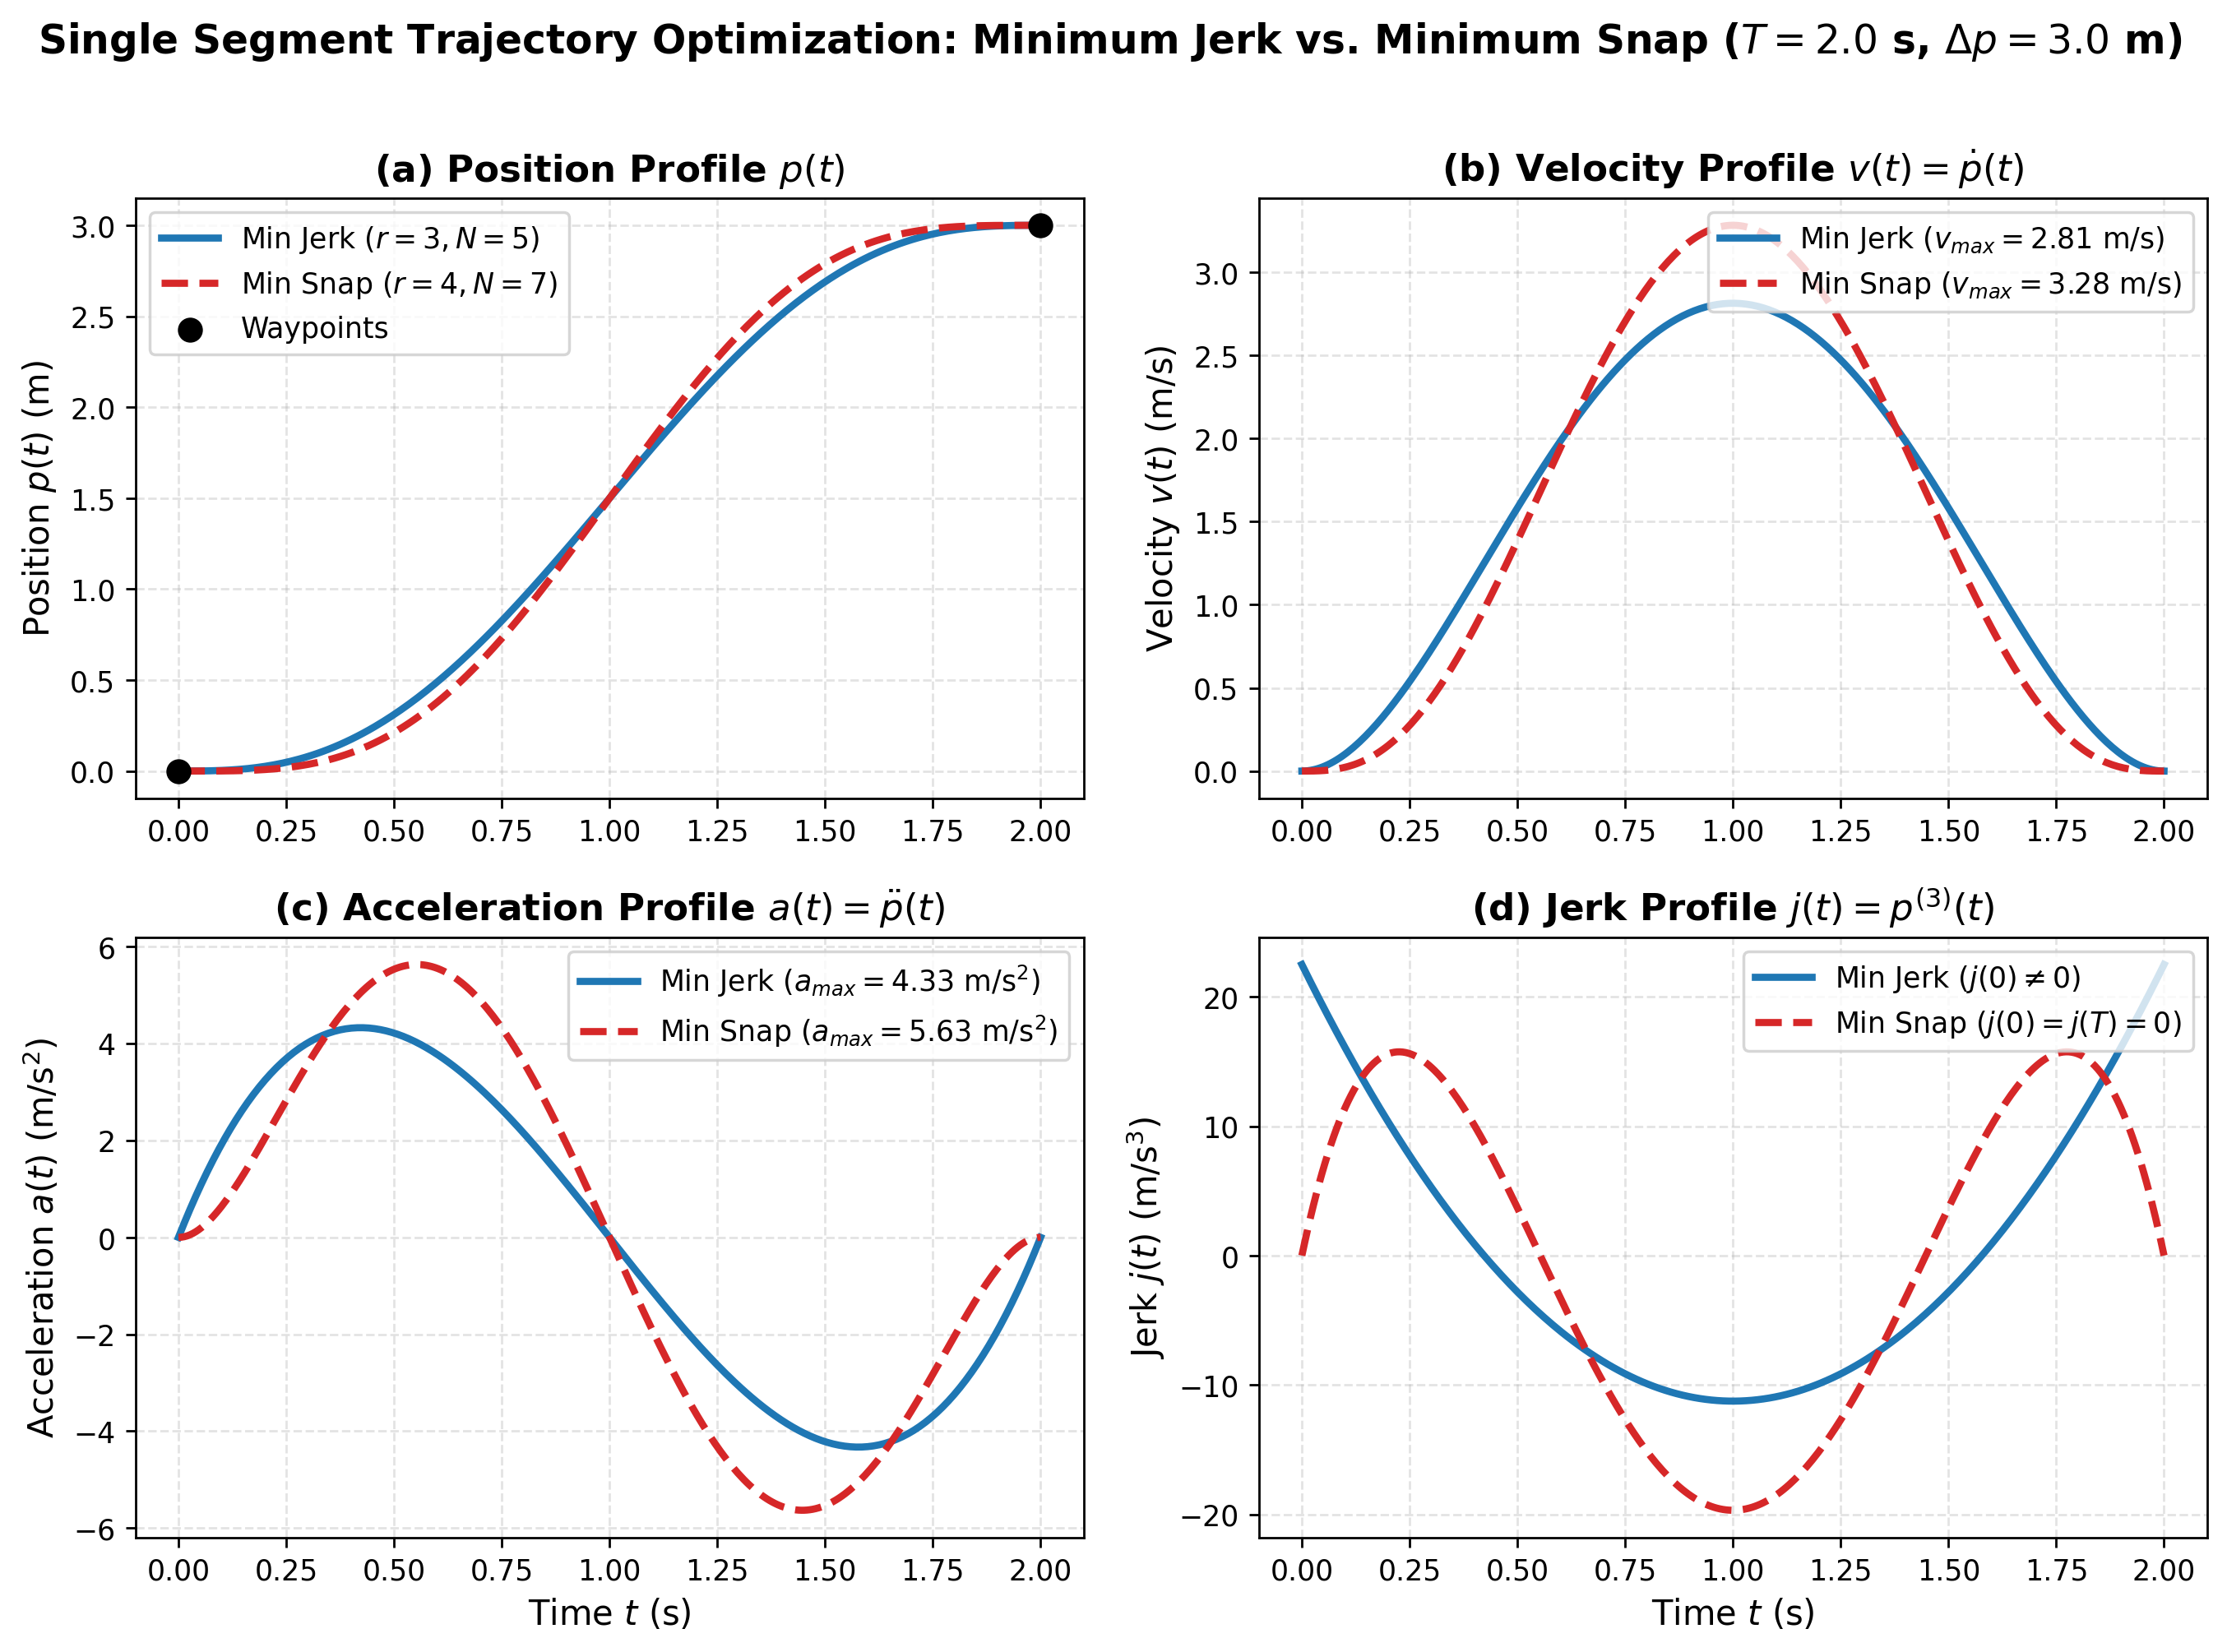
\includegraphics[width=0.95\textwidth]{single_segment_profiles.png}
    \caption{\textbf{Single Segment Trajectory Comparison}: Minimum Jerk ($r=3, N=5$) vs. Minimum Snap ($r=4, N=7$) for $T=2.0\,\text{s}$ and displacement $\Delta p = 3.0\,\text{m}$. Notice that Minimum Snap guarantees zero jerk at the boundaries ($j(0) = j(T) = 0$), preventing discontinuous rotational torque shocks at takeoff and touchdown, at the expense of slightly higher peak velocity and acceleration.}
    \caption{\textbf{Single Segment Trajectory Comparison}: Minimum Jerk ($r=3, N=5$) vs. Minimum Snap ($r=4, N=7$) for $T=2.0\,\text{s}$ and displacement $\Delta p = 3.0\,\text{m}$. Minimum snap guarantees zero jerk at the boundaries ($j(0) = j(T) = 0$), preventing discontinuous rotational torque shocks at takeoff and touchdown, at the expense of slightly higher peak velocity and acceleration.}
    \label{fig:single_segment_profiles}
\end{figure}

% =============================================================================
\section{End-to-End Concrete Example: Quintic Minimum Jerk Polynomial}
% =============================================================================

We now present a complete, step-by-step worked example. We choose the canonical **minimum jerk polynomial ($r=3$)** with **order $N=5$ (quintic polynomial)**, explicitly deriving and populating both the Hessian matrix and the constraint matrix, assembling the KKT system, and solving it in closed form.

\subsection{Why the Quintic Polynomial is the Appropriate Choice}

In 3D quadrotor flight, a smooth maneuver requires matching initial and final states:
\begin{itemize}
    \item At $t=0$: position $p(0) = p_0$, velocity $\dot{p}(0) = v_0$, acceleration $\ddot{p}(0) = a_0$ (3 conditions).
    \item At $t=T$: position $p(T) = p_f$, velocity $\dot{p}(T) = v_f$, acceleration $\ddot{p}(T) = a_f$ (3 conditions).
\end{itemize}
This gives a total of $m = 6$ boundary equality constraints. An $N$-th order polynomial:
\begin{equation}
p(t) = c_0 + c_1 t + c_2 t^2 + c_3 t^3 + c_4 t^4 + c_5 t^5
\end{equation}
has $N+1 = 6$ unknown coefficients $\mathbf{c} = [c_0, c_1, c_2, c_3, c_4, c_5]^T \in \mathbb{R}^6$. Thus, $N=5$ is the exact minimal polynomial order that can satisfy all boundary conditions for minimum jerk.

\subsection{Step 1: Constructing the Hessian Matrix \texorpdfstring{$\mathbf{Q}(T)$}{Q(T)}}

The jerk is the 3rd time derivative of $p(t)$:
\begin{equation}
p^{(3)}(t) = 6 c_3 + 24 c_4 t + 60 c_5 t^2
\end{equation}
The integrand of the objective cost is the squared jerk:
\begin{align}
\left( p^{(3)}(t) \right)^2 &= \left( 6 c_3 + 24 c_4 t + 60 c_5 t^2 \right)^2 \nonumber \\
&= 36 c_3^2 + 288 c_3 c_4 t + \left( 576 c_4^2 + 720 c_3 c_5 \right) t^2 + 2880 c_4 c_5 t^3 + 3600 c_5^2 t^4
\end{align}
Integrating term-by-term from $t=0$ to $t=T$:
\begin{equation}
J = \int_0^T \left( p^{(3)}(t) \right)^2 dt
= 36 T c_3^2 + 144 T^2 c_3 c_4 + 240 T^3 c_3 c_5 + 192 T^3 c_4^2 + 720 T^4 c_4 c_5 + 720 T^5 c_5^2
\end{equation}
Writing this in matrix quadratic form $J = \mathbf{c}^T \mathbf{Q}(T) \mathbf{c}$:
\begin{equation}
\label{eq:Q_quintic_symbolic}
\mathbf{Q}(T) = \begin{bmatrix}
0 & 0 & 0 & 0 & 0 & 0 \\
0 & 0 & 0 & 0 & 0 & 0 \\
0 & 0 & 0 & 0 & 0 & 0 \\
0 & 0 & 0 & 36 T & 72 T^2 & 120 T^3 \\
0 & 0 & 0 & 72 T^2 & 192 T^3 & 360 T^4 \\
0 & 0 & 0 & 120 T^3 & 360 T^4 & 720 T^5
\end{bmatrix} \in \mathbb{R}^{6 \times 6}
\end{equation}
The QP objective matrix $\mathbf{P} = 2 \mathbf{Q}(T)$ is therefore:
\begin{equation}
\label{eq:P_quintic_symbolic}
\mathbf{P} = \begin{bmatrix}
0 & 0 & 0 & 0 & 0 & 0 \\
0 & 0 & 0 & 0 & 0 & 0 \\
0 & 0 & 0 & 0 & 0 & 0 \\
0 & 0 & 0 & 72 T & 144 T^2 & 240 T^3 \\
0 & 0 & 0 & 144 T^2 & 384 T^3 & 720 T^4 \\
0 & 0 & 0 & 240 T^3 & 720 T^4 & 1440 T^5
\end{bmatrix}
\end{equation}

\subsection{Step 2: Constructing the Equality Constraint Matrix \texorpdfstring{$\mathbf{A}(T)$}{A(T)}}

We express the boundary conditions in terms of the basis derivatives:
\begin{align}
p(0) &= c_0 = p_0 \\
\dot{p}(0) &= c_1 = v_0 \\
\ddot{p}(0) &= 2 c_2 = a_0 \\
p(T) &= c_0 + c_1 T + c_2 T^2 + c_3 T^3 + c_4 T^4 + c_5 T^5 = p_f \\
\dot{p}(T) &= c_1 + 2 c_2 T + 3 c_3 T^2 + 4 c_4 T^3 + 5 c_5 T^4 = v_f \\
\ddot{p}(T) &= 2 c_2 + 6 c_3 T + 12 c_4 T^2 + 20 c_5 T^3 = a_f
\end{align}
In matrix form $\mathbf{A}(T) \mathbf{c} = \mathbf{b}$:
\begin{equation}
\label{eq:A_quintic_symbolic}
\mathbf{A}(T) = \begin{bmatrix}
1 & 0 & 0 & 0 & 0 & 0 \\
0 & 1 & 0 & 0 & 0 & 0 \\
0 & 0 & 2 & 0 & 0 & 0 \\
1 & T & T^2 & T^3 & T^4 & T^5 \\
0 & 1 & 2T & 3T^2 & 4T^3 & 5T^4 \\
0 & 0 & 2 & 6T & 12T^2 & 20T^3
\end{bmatrix}, \qquad
\mathbf{b} = \begin{bmatrix}
p_0 \\ v_0 \\ a_0 \\ p_f \\ v_f \\ a_f
\end{bmatrix}
\end{equation}

\subsection{Step 3: Numerical Instantiation and Closed-Form Solve}

Let us solve a realistic rest-to-rest flight maneuver:
\begin{itemize}
    \item Duration: $T = 2.0\,\text{s}$
    \item Start: $p_0 = 0.0\,\text{m}$, $v_0 = 0.0\,\text{m/s}$, $a_0 = 0.0\,\text{m/s}^2$
    \item Goal: $p_f = 3.0\,\text{m}$, $v_f = 0.0\,\text{m/s}$, $a_f = 0.0\,\text{m/s}^2$
\end{itemize}
The constraint vector is:
\begin{equation}
\mathbf{b} = \begin{bmatrix} 0 & 0 & 0 & 3 & 0 & 0 \end{bmatrix}^T
\end{equation}
Evaluating $\mathbf{Q}(T)$, $\mathbf{P} = 2\mathbf{Q}(T)$, and $\mathbf{A}(T)$ at $T = 2.0$:
\begin{equation}
\mathbf{Q}(2) = \begin{bmatrix}
0 & 0 & 0 & 0 & 0 & 0 \\
0 & 0 & 0 & 0 & 0 & 0 \\
0 & 0 & 0 & 0 & 0 & 0 \\
0 & 0 & 0 & 72 & 288 & 960 \\
0 & 0 & 0 & 288 & 1536 & 5760 \\
0 & 0 & 0 & 960 & 5760 & 23040
\end{bmatrix}, \qquad
\mathbf{A}(2) = \begin{bmatrix}
1 & 0 & 0 & 0 & 0 & 0 \\
0 & 1 & 0 & 0 & 0 & 0 \\
0 & 0 & 2 & 0 & 0 & 0 \\
1 & 2 & 4 & 8 & 16 & 32 \\
0 & 1 & 4 & 12 & 32 & 80 \\
0 & 0 & 2 & 12 & 48 & 160
\end{bmatrix}
\end{equation}
The full $12 \times 12$ KKT system is:
\begin{equation}
\begin{bmatrix}
2\mathbf{Q}(2) & \mathbf{A}(2)^T \\
\mathbf{A}(2) & \mathbf{0}_{6 \times 6}
\end{bmatrix}
\begin{bmatrix}
\mathbf{c}^* \\
\boldsymbol{\nu}^*
\end{bmatrix}
=
\begin{bmatrix}
\mathbf{0}_{6 \times 1} \\
\mathbf{b}
\end{bmatrix}
\end{equation}
Solving this linear system yields the exact analytical optimal solution:
\begin{equation}
\mathbf{c}^* = \begin{bmatrix}
c_0^* \\ c_1^* \\ c_2^* \\ c_3^* \\ c_4^* \\ c_5^*
\end{bmatrix}
=
\begin{bmatrix}
0 \\ 0 \\ 0 \\ 3.75 \\ -2.8125 \\ 0.5625
\end{bmatrix}
=
\begin{bmatrix}
0 \\ 0 \\ 0 \\ \frac{15}{4} \\ -\frac{45}{16} \\ \frac{9}{16}
\end{bmatrix}, \qquad
\boldsymbol{\nu}^* =
\begin{bmatrix}
135 \\ 135 \\ 45 \\ -135 \\ 135 \\ -45
\end{bmatrix}
\end{equation}
The continuous position trajectory is therefore:
\begin{equation}
p(t) = \frac{15}{4} t^3 - \frac{45}{16} t^4 + \frac{9}{16} t^5
\end{equation}
Differentiating to find velocity, acceleration, and jerk:
\begin{align}
v(t) &= \dot{p}(t) = \frac{45}{4} t^2 - \frac{45}{4} t^3 + \frac{45}{16} t^4 \\
a(t) &= \ddot{p}(t) = \frac{45}{2} t - \frac{135}{4} t^2 + \frac{45}{4} t^3 \\
j(t) &= p^{(3)}(t) = \frac{45}{2} - \frac{135}{2} t + \frac{135}{4} t^2
\end{align}
Notice that:
\begin{itemize}
    \item At $t=0$: $p(0) = 0$, $v(0) = 0$, $a(0) = 0$.
    \item At $t=2$: $p(2) = \frac{15}{4}(8) - \frac{45}{16}(16) + \frac{9}{16}(32) = 30 - 45 + 18 = 3.0\,\text{m}$.
    \item At $t=2$: $v(2) = \frac{45}{4}(4) - \frac{45}{4}(8) + \frac{45}{16}(16) = 45 - 90 + 45 = 0.0\,\text{m/s}$.
    \item At $t=2$: $a(2) = \frac{45}{2}(2) - \frac{135}{4}(4) + \frac{45}{4}(8) = 45 - 135 + 90 = 0.0\,\text{m/s}^2$.
\end{itemize}
The cumulative objective jerk cost evaluated analytically is:
\begin{equation}
J^* = \mathbf{c}^{*T} \mathbf{Q}(2) \mathbf{c}^* = \frac{405}{2} = 202.5
\end{equation}

\subsection{Over-Parameterized Example (\texorpdfstring{$N=6$}{N=6}, 7 Coefficients, 6 Constraints)}

What occurs if we deliberately select a polynomial of degree $N=6$ ($7$ unknown coefficients) while enforcing the same $6$ boundary conditions?
The constraint matrix $\mathbf{A} \in \mathbb{R}^{6 \times 7}$ now has a $1$-dimensional nullspace. The KKT system has dimension $(7 + 6) \times (7 + 6) = 13 \times 13$:
\begin{equation}
\begin{bmatrix}
2\mathbf{Q}_{7 \times 7}(2) & \mathbf{A}_{6 \times 7}^T \\
\mathbf{A}_{6 \times 7} & \mathbf{0}_{6 \times 6}
\end{bmatrix}
\begin{bmatrix}
\mathbf{c}^* \\
\boldsymbol{\nu}^*
\end{bmatrix}
=
\begin{bmatrix}
\mathbf{0}_{7 \times 1} \\
\mathbf{b}_{6 \times 1}
\end{bmatrix}
\end{equation}
Solving this $13 \times 13$ system yields:
\begin{equation}
\mathbf{c}^* = \begin{bmatrix} 0 & 0 & 0 & 3.75 & -2.8125 & 0.5625 & \mathbf{0.0} \end{bmatrix}^T
\end{equation}
The optimization automatically zeroes out the 6th coefficient $c_6^* = 0$. This confirms the fundamental Euler-Lagrange theorem: the minimum jerk trajectory connecting 6 boundary conditions is strictly quintic.

\subsection{Python Code: Analytical KKT Inversion vs. CVXOPT}

The following self-contained script confirms that the closed-form KKT matrix inverse and CVXOPT produce identical solutions:

\begin{lstlisting}[language=Python, caption={Closed-Form KKT vs. CVXOPT for Quintic Minimum Jerk.}]
import numpy as np
import cvxopt
from cvxopt import matrix, solvers
solvers.options['show_progress'] = False

T, p0, pf = 2.0, 0.0, 3.0

# 1. Hessian Q(2) for N=5, r=3
Q = np.zeros((6, 6))
Q[3, 3] = 36 * T;          Q[3, 4] = 72 * T**2;      Q[3, 5] = 120 * T**3
Q[4, 3] = 72 * T**2;       Q[4, 4] = 192 * T**3;     Q[4, 5] = 360 * T**4
Q[5, 3] = 120 * T**3;      Q[5, 4] = 360 * T**4;     Q[5, 5] = 720 * T**5

# 2. Constraint matrix A(2) and vector b
A = np.array([
    [1, 0, 0, 0, 0, 0],
    [0, 1, 0, 0, 0, 0],
    [0, 0, 2, 0, 0, 0],
    [1, T, T**2, T**3, T**4, T**5],
    [0, 1, 2*T, 3*T**2, 4*T**3, 5*T**4],
    [0, 0, 2, 6*T, 12*T**2, 20*T**3]
], dtype=float)
b = np.array([p0, 0.0, 0.0, pf, 0.0, 0.0])

# 3. Method A: Closed-Form KKT Matrix Inversion
K = np.block([[2.0 * Q, A.T], [A, np.zeros((6, 6))]])
rhs = np.concatenate([np.zeros(6), b])
sol_kkt = np.linalg.solve(K, rhs)
c_kkt = sol_kkt[:6]

# 4. Method B: Numerical Solve via CVXOPT
P_cvx = matrix(2.0 * Q)
q_cvx = matrix(np.zeros(6))
A_cvx = matrix(A)
b_cvx = matrix(b)
sol_cvx = solvers.qp(P_cvx, q_cvx, None, None, A_cvx, b_cvx)
c_cvx = np.array(sol_cvx['x']).flatten()

print("Closed-form c*:", np.round(c_kkt, 6))
print("CVXOPT      c*:", np.round(c_cvx, 6))
# Both print: [ 0.  0.  0.  3.75 -2.8125 0.5625]
\end{lstlisting}

% =============================================================================
\section{Impact of Varying the Time Interval \texorpdfstring{$T$}{T}}
\label{sec:time_scaling}
% =============================================================================

A critical practical question in quadrotor motion planning is: \emph{How should the segment duration $T$ be chosen?} In this section, we analyze the impact of varying $T$ both analytically and empirically.

\subsection{Analytical Cost Scaling Law: \texorpdfstring{$J^*(T) \propto T^{-(2r-1)}$}{J*(T) proportional to T\textasciicircum(-(2r-1))}}

To understand how duration affects optimal cost, consider non-dimensionalizing time. Define the normalized time variable:
To understand how duration affects optimal cost, define the normalized time variable:
\begin{equation}
\tau \triangleq \frac{t}{T} \in [0, 1] \implies dt = T \, d\tau
\end{equation}
Let $\tilde{p}(\tau) \triangleq p(T\tau)$ denote the trajectory parameterized on the unit interval $[0, 1]$. By the chain rule:
\begin{equation}
\frac{d^r p(t)}{dt^r} = \frac{1}{T^r} \frac{d^r \tilde{p}(\tau)}{d\tau^r}
\end{equation}
Now, substitute this expression into the objective function:
Substitute this expression into the objective function:
\begin{align}
J &= \int_0^T \left( \frac{d^r p(t)}{dt^r} \right)^2 dt \\
  &= \int_0^1 \left( \frac{1}{T^r} \frac{d^r \tilde{p}(\tau)}{d\tau^r} \right)^2 (T \, d\tau) \\
  &= \frac{1}{T^{2r - 1}} \int_0^1 \left( \frac{d^r \tilde{p}(\tau)}{d\tau^r} \right)^2 d\tau
\end{align}
Because the normalized profile $\tilde{p}(\tau)$ satisfies fixed boundary conditions (such as $\tilde{p}(0)=p_0$, $\tilde{p}(1)=p_f$), the integral $\tilde{J} \triangleq \int_0^1 (\tilde{p}^{(r)})^2 d\tau$ depends only on the spatial displacement $\Delta p = p_f - p_0$, not on $T$.

\begin{definitionbox}[Fundamental Scaling Laws for Polynomial Trajectories]
For a rest-to-rest displacement $\Delta p$ over duration $T$:
\begin{enumerate}
    \item \textbf{Optimal Objective Cost}:
    \begin{equation}
    J^*(T) \propto \frac{\Delta p^2}{T^{2r - 1}}
    \end{equation}
    \begin{itemize}
        \item Minimum Acceleration ($r=2$): $J^*(T) \propto T^{-3}$
        \item Minimum Jerk ($r=3$): $J^*(T) \propto T^{-5}$
        \item Minimum Jerk ($r=3$): $J^*(T) = \dfrac{720 \, \Delta p^2}{T^5} \propto T^{-5}$
        \item Minimum Snap ($r=4$): $J^*(T) \propto T^{-7}$
    \end{itemize}
    \item \textbf{Peak Kinematic States}:
    \begin{align}
    v_{\max}(T) &\propto \frac{\Delta p}{T} \quad (T^{-1}) \\[0.4em]
    a_{\max}(T) &\propto \frac{\Delta p}{T^2} \quad (T^{-2}) \\[0.4em]
    j_{\max}(T) &\propto \frac{\Delta p}{T^3} \quad (T^{-3})
    \end{align}
\end{enumerate}
\end{definitionbox}

\begin{figure}[H]
    \centering
    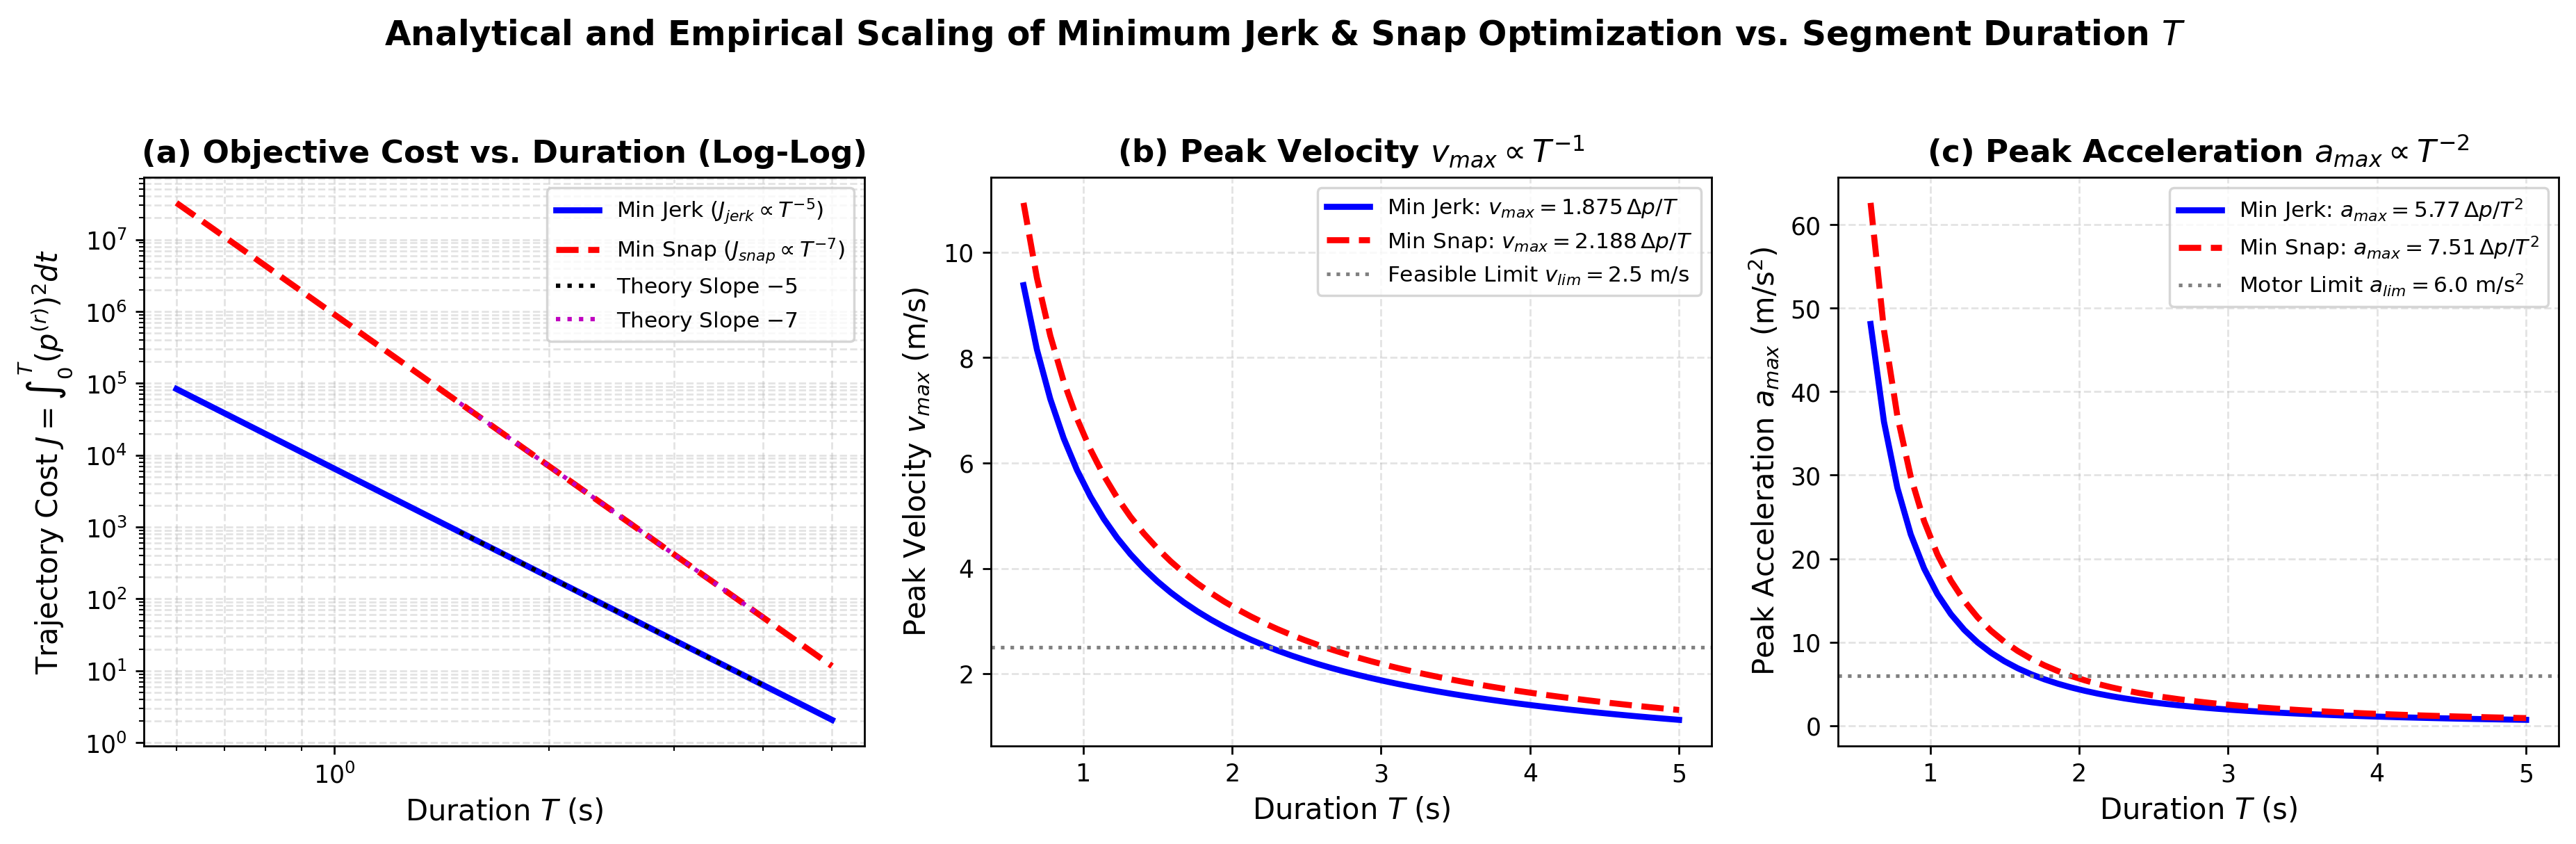
\includegraphics[width=0.98\textwidth]{time_scaling_analysis.png}
    \caption{\textbf{Analytical and Empirical Scaling vs. Duration $T$}: 
    \textbf{(a)} Log-log plot of objective cost $J(T)$ against $T$. The slopes precisely match the theoretical exponents $-5$ for minimum jerk and $-7$ for minimum snap.
    \textbf{(b)} Peak velocity scaling as $v_{\max} \propto 1/T$.
    \textbf{(c)} Peak acceleration scaling as $a_{\max} \propto 1/T^2$. The dotted lines indicate physical actuator limits ($v_{\lim}=2.5\,\text{m/s}$, $a_{\lim}=6.0\,\text{m/s}^2$), defining the minimum feasible duration $T_{\min}$.}
    \label{fig:time_scaling_analysis}
\end{figure}

\subsection{The Flight Time vs. Actuation Trade-Off}

The steep power-law dependencies on $T$ establish a critical trade-off:
\begin{itemize}
    \item \textbf{Small $T$ ($T \to 0$)}: Trajectory cost explodes exponentially ($T^{-5}$ or $T^{-7}$). More critically, required accelerations and jerks exceed physical motor capabilities ($a_{\max} \propto T^{-2}$, $j_{\max} \propto T^{-3}$). The quadrotor encounters thrust saturation, rotor stall, or severe attitude tracking errors.
    \item \textbf{Small $T$ ($T \to 0$)}: Trajectory cost explodes rapidly ($T^{-5}$ or $T^{-7}$). More critically, required accelerations and jerks exceed physical motor capabilities ($a_{\max} \propto T^{-2}$, $j_{\max} \propto T^{-3}$). The quadrotor encounters thrust saturation, rotor stall, or severe attitude tracking errors.
    \item \textbf{Large $T$ ($T \to \infty$)}: Trajectory cost vanishes toward zero, and required motor efforts become negligible. However, mission transit time is unnecessarily long, leaving the quadrotor susceptible to wind gusts and drift.
\end{itemize}

\begin{table}[H]
\centering
\caption{\textbf{Numerical Comparison of Trajectory Metrics as Duration $T$ Varies} ($\Delta p = 3.0\,\text{m}$, Rest-to-Rest, Minimum Jerk $N=5, r=3$ vs. Minimum Snap $N=7, r=4$).}
\vspace{0.5em}
\resizebox{\textwidth}{!}{%
\begin{tabular}{@{}ccccccc@{}}
\toprule
\textbf{Duration $T$ (s)} & \multicolumn{2}{c}{\textbf{Objective Cost $J^*(T)$}} & \multicolumn{2}{c}{\textbf{Peak Velocity $v_{\max}$ (m/s)}} & \multicolumn{2}{c}{\textbf{Peak Acceleration $a_{\max}$ (m/s$^2$)}} \\
\cmidrule(lr){2-3} \cmidrule(lr){4-5} \cmidrule(lr){6-7}
 & \textbf{Min Jerk} & \textbf{Min Snap} & \textbf{Min Jerk} & \textbf{Min Snap} & \textbf{Min Jerk} & \textbf{Min Snap} \\
\midrule
$0.6$ & $91{,}125$ & $33{,}067{,}407$ & $9.38$ & $10.94$ & $48.11$ & $62.59$ \\
$1.0$ & $7{,}088$ & $1{,}210{,}050$ & $5.62$ & $6.56$ & $17.32$ & $22.53$ \\
$1.5$ & $933$ & $70{,}794$ & $3.75$ & $4.38$ & $7.70$ & $10.01$ \\
$2.0$ & $221$ & $9{,}453$ & $2.81$ & $3.28$ & $4.33$ & $5.63$ \\
$3.0$ & $29.2$ & $447$ & $1.87$ & $2.19$ & $1.92$ & $2.50$ \\
$4.0$ & $6.9$ & $42.6$ & $1.41$ & $1.64$ & $1.08$ & $1.41$ \\
$5.0$ & $2.3$ & $8.9$ & $1.12$ & $1.31$ & $0.69$ & $0.90$ \\
$2.0$ & $202.5$ & $9{,}453$ & $2.81$ & $3.28$ & $4.33$ & $5.63$ \\
$3.0$ & $26.7$ & $447$ & $1.87$ & $2.19$ & $1.92$ & $2.50$ \\
$4.0$ & $6.3$ & $42.6$ & $1.41$ & $1.64$ & $1.08$ & $1.41$ \\
$5.0$ & $2.1$ & $8.9$ & $1.12$ & $1.31$ & $0.69$ & $0.90$ \\
\bottomrule
\end{tabular}%
}
\label{tab:time_sweep_results}
\end{table}

\begin{figure}[H]
    \centering
    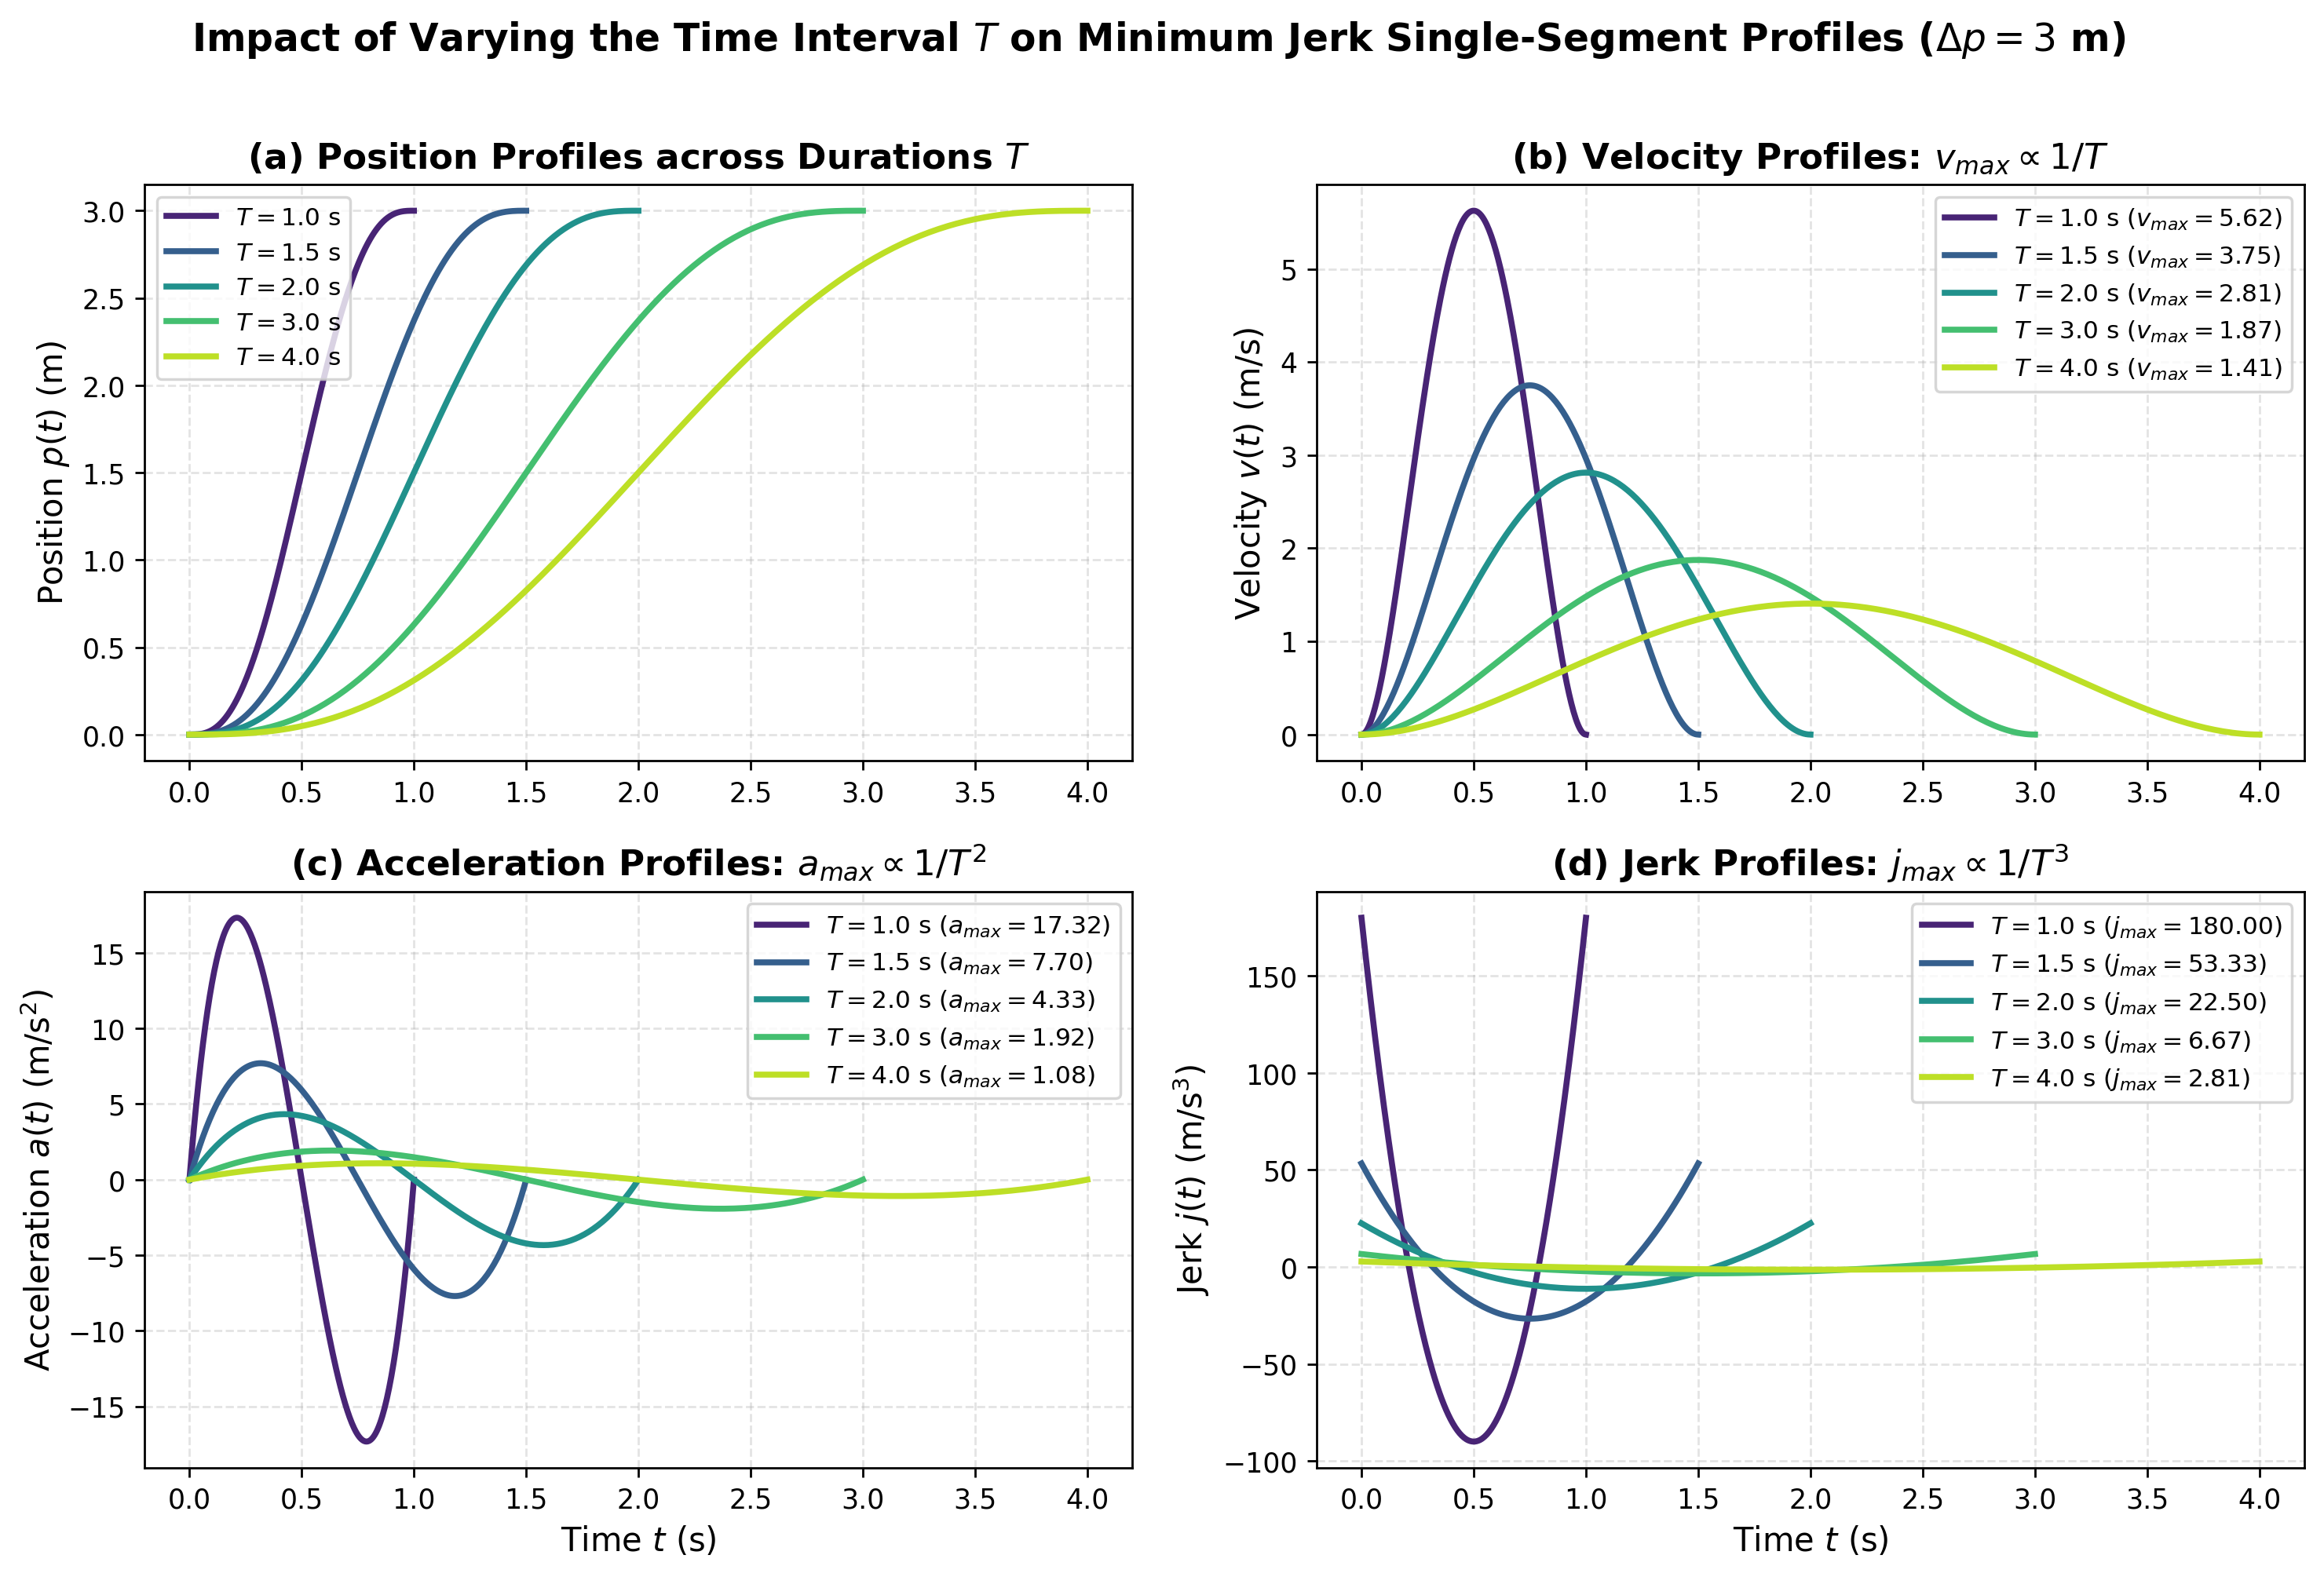
\includegraphics[width=0.98\textwidth]{time_interval_sweep.png}
    \caption{\textbf{Effect of Segment Duration $T$ on Minimum Jerk Profiles}: Position, velocity, acceleration, and jerk profiles for $T \in \{1.0, 1.5, 2.0, 3.0, 4.0\}\,\text{s}$. Shortening the duration from $4.0\,\text{s}$ to $1.0\,\text{s}$ increases peak acceleration sixteen-fold ($1.08 \to 17.32\,\text{m/s}^2$) and peak jerk sixty-four-fold ($2.81 \to 180.0\,\text{m/s}^3$).}
    \label{fig:time_interval_sweep}
\end{figure}

\subsection{Actuator Feasibility and Optimal Duration Selection}

A physical quadrotor with maximum collective thrust $f_{\max}$ has an acceleration limit $a_{\lim} \approx \frac{f_{\max}}{m} - g$ and a maximum safe cruise speed $v_{\lim}$. From Table~\ref{tab:time_sweep_results} and the analytical formulas:
\begin{equation}
v_{\max} = c_v \frac{\Delta p}{T}, \qquad a_{\max} = c_a \frac{\Delta p}{T^2}
\end{equation}
where for minimum jerk $c_v = 1.875, c_a = 5.774$, and for minimum snap $c_v = 2.188, c_a = 7.513$.

To guarantee that the trajectory respects physical hardware limits, the segment duration must satisfy:
To guarantee that the trajectory respects physical hardware limits without needing inequality constraints, the segment duration is selected analytically:
\begin{equation}
T \ge T_{\min} \triangleq \max\left( \frac{c_v \Delta p}{v_{\lim}}, \; \sqrt{\frac{c_a \Delta p}{a_{\lim}}} \right)
\end{equation}
In practical trajectory generation pipelines, setting $T = 1.15 \times T_{\min}$ to $1.30 \times T_{\min}$ provides a robust safety margin against aerodynamic disturbances and unmodeled drag.

% =============================================================================
\section{Multi-Waypoint Trajectory Planning via Piecewise Polynomial QP}
\section{Multi-Waypoint Trajectory Planning via Piecewise Polynomial EQP}
% =============================================================================

Real-world drone missions require traversing sequences of waypoints (e.g., inspecting building facades, navigating warehouse aisles, or flying through obstacle corridors). While one might attempt to fit a single high-degree polynomial through all waypoints, this approach suffers from severe numerical ill-conditioning (Runge's phenomenon) and cannot independently allocate time to different flight segments.
Real-world drone missions require traversing sequences of waypoints (e.g., inspecting building facades, navigating warehouse corridors, or flying through survey waypoints). Fitting a single high-degree polynomial through all waypoints causes severe numerical ill-conditioning (Runge's phenomenon) and cannot independently allocate time to different flight segments.

The standard solution is \textbf{piecewise polynomial trajectory planning}.

\subsection{Piecewise Formulation}

Consider a mission with $M+1$ ordered waypoints $\mathbf{w}_0, \mathbf{w}_1, \dots, \mathbf{w}_M \in \mathbb{R}^3$ partitioned into $M$ sequential segments. Each segment $m \in \{1, \dots, M\}$ has duration $T_m > 0$. We express time in segment $m$ using a local clock:
\begin{equation}
\tau_m \triangleq t - t_{m-1} \in [0, T_m], \qquad \text{where } t_0 = 0, \quad t_m = \sum_{k=1}^m T_k
\end{equation}
The trajectory in segment $m$ along a single coordinate axis is:
\begin{equation}
p_m(\tau_m) = \sum_{k=0}^N c_{m, k} \tau_m^k = \mathbf{t}(\tau_m)^T \mathbf{c}_m, \qquad \mathbf{c}_m \in \mathbb{R}^{N+1}
\end{equation}
The total decision vector $\mathbf{c} \in \mathbb{R}^{M(N+1)}$ stacks the coefficients of all $M$ segments:
\begin{equation}
\mathbf{c} = \begin{bmatrix} \mathbf{c}_1 \\ \mathbf{c}_2 \\ \vdots \\ \mathbf{c}_M \end{bmatrix} \in \mathbb{R}^{M(N+1)}
\end{equation}

\subsection{Total Objective Function}

The cumulative cost over the entire multi-segment mission is the sum of the individual segment costs:
\begin{equation}
J_{\text{total}} = \sum_{m=1}^M \int_0^{T_m} \left( p_m^{(r)}(\tau_m) \right)^2 d\tau_m
= \sum_{m=1}^M \mathbf{c}_m^T \mathbf{Q}_m(T_m) \mathbf{c}_m
\end{equation}
where $\mathbf{Q}_m(T_m)$ is computed using the analytical formula in Eq.~\eqref{eq:Q_formula} with $T = T_m$.

In block matrix form:
\begin{equation}
J_{\text{total}} = \mathbf{c}^T \mathbf{Q}_{\text{total}} \mathbf{c}, \qquad
\mathbf{Q}_{\text{total}} = \begin{bmatrix}
\mathbf{Q}_1(T_1) & \mathbf{0} & \dots & \mathbf{0} \\
\mathbf{0} & \mathbf{Q}_2(T_2) & \dots & \mathbf{0} \\
\vdots & \vdots & \ddots & \vdots \\
\mathbf{0} & \mathbf{0} & \dots & \mathbf{Q}_M(T_M)
\end{bmatrix}
\end{equation}
Thus, the objective matrix in standard QP form is block-diagonal:
\begin{equation}
\mathbf{P} = 2 \, \mathbf{Q}_{\text{total}} \in \mathbb{R}^{M(N+1) \times M(N+1)}, \qquad \mathbf{q} = \mathbf{0}_{M(N+1) \times 1}
\end{equation}

\subsection{Multi-Segment Equality Constraints}

The linear equality constraint system $\mathbf{A}_{eq} \mathbf{c} = \mathbf{b}_{eq}$ encapsulates three physical requirements:
The linear equality constraint system $\mathbf{A} \mathbf{c} = \mathbf{b}$ encapsulates three physical requirements:

\subsubsection{1. Waypoint Passage Constraints}
Every segment $m \in \{1, \dots, M\}$ must start at waypoint $\mathbf{w}_{m-1}$ and end at waypoint $\mathbf{w}_m$:
\begin{align}
p_m(0) &= \mathbf{t}^{(0)}(0)^T \mathbf{c}_m = w_{m-1} \\
p_m(T_m) &= \mathbf{t}^{(0)}(T_m)^T \mathbf{c}_m = w_m
\end{align}
This contributes $2M$ scalar equality constraints.

\subsubsection{2. Inter-Segment Continuity Constraints (\texorpdfstring{$C^k$}{C\textasciicircum k} Smoothness)}
At each internal junction $m \in \{1, \dots, M-1\}$, the trajectory must transition smoothly. Derivatives of order $d = 1, \dots, r$ must match across the boundary:
\begin{equation}
p_m^{(d)}(T_m) = p_{m+1}^{(d)}(0)
\implies
\mathbf{t}^{(d)}(T_m)^T \mathbf{c}_m - \mathbf{t}^{(d)}(0)^T \mathbf{c}_{m+1} = 0
\end{equation}
For minimum snap ($r=4$), enforcing continuity for $d \in \{1, 2, 3, 4\}$ ensures continuity of velocity ($C^1$), acceleration ($C^2$), jerk ($C^3$), and snap ($C^4$). This contributes $r(M-1)$ scalar equality constraints.

\subsubsection{3. Initial and Terminal Mission Boundaries}
At the start of the mission ($t=0$, segment 1) and at the completion ($t=t_{\text{final}}$, segment $M$), the quadrotor typically starts and ends at hover:
\begin{align}
p_1^{(d)}(0) &= 0, \quad \forall d \in \{1, \dots, r-1\} \\
p_M^{(d)}(T_M) &= 0, \quad \forall d \in \{1, \dots, r-1\}
\end{align}
This contributes $2(r-1)$ scalar equality constraints.

\begin{intuitionbox}[Decoupling of Spatial Coordinates]
Notice that in the above equations, the constraints and cost functions for $x(t)$, $y(t)$, and $z(t)$ share the \textbf{exact same} $\mathbf{P}$ and $\mathbf{A}_{eq}$ matrices! Only the right-hand side vector $\mathbf{b}_{eq}$ changes to reflect the corresponding waypoint coordinates ($w_{x, m}, w_{y, m}, w_{z, m}$).
In the multi-segment formulation, the constraint matrix $\mathbf{A}$ and Hessian $\mathbf{P}$ for $x(t)$, $y(t)$, and $z(t)$ are \textbf{identical}. Only the right-hand side vector $\mathbf{b}$ changes to reflect the corresponding waypoint coordinates ($w_{x, m}, w_{y, m}, w_{z, m}$).

Consequently, the 3D trajectory problem decomposes into \textbf{three independent 1D QPs} that can be solved in parallel.
Consequently, the 3D trajectory problem decomposes into \textbf{three independent 1D EQPs} that can be solved in parallel.
\end{intuitionbox}

\begin{figure}[H]
    \centering
    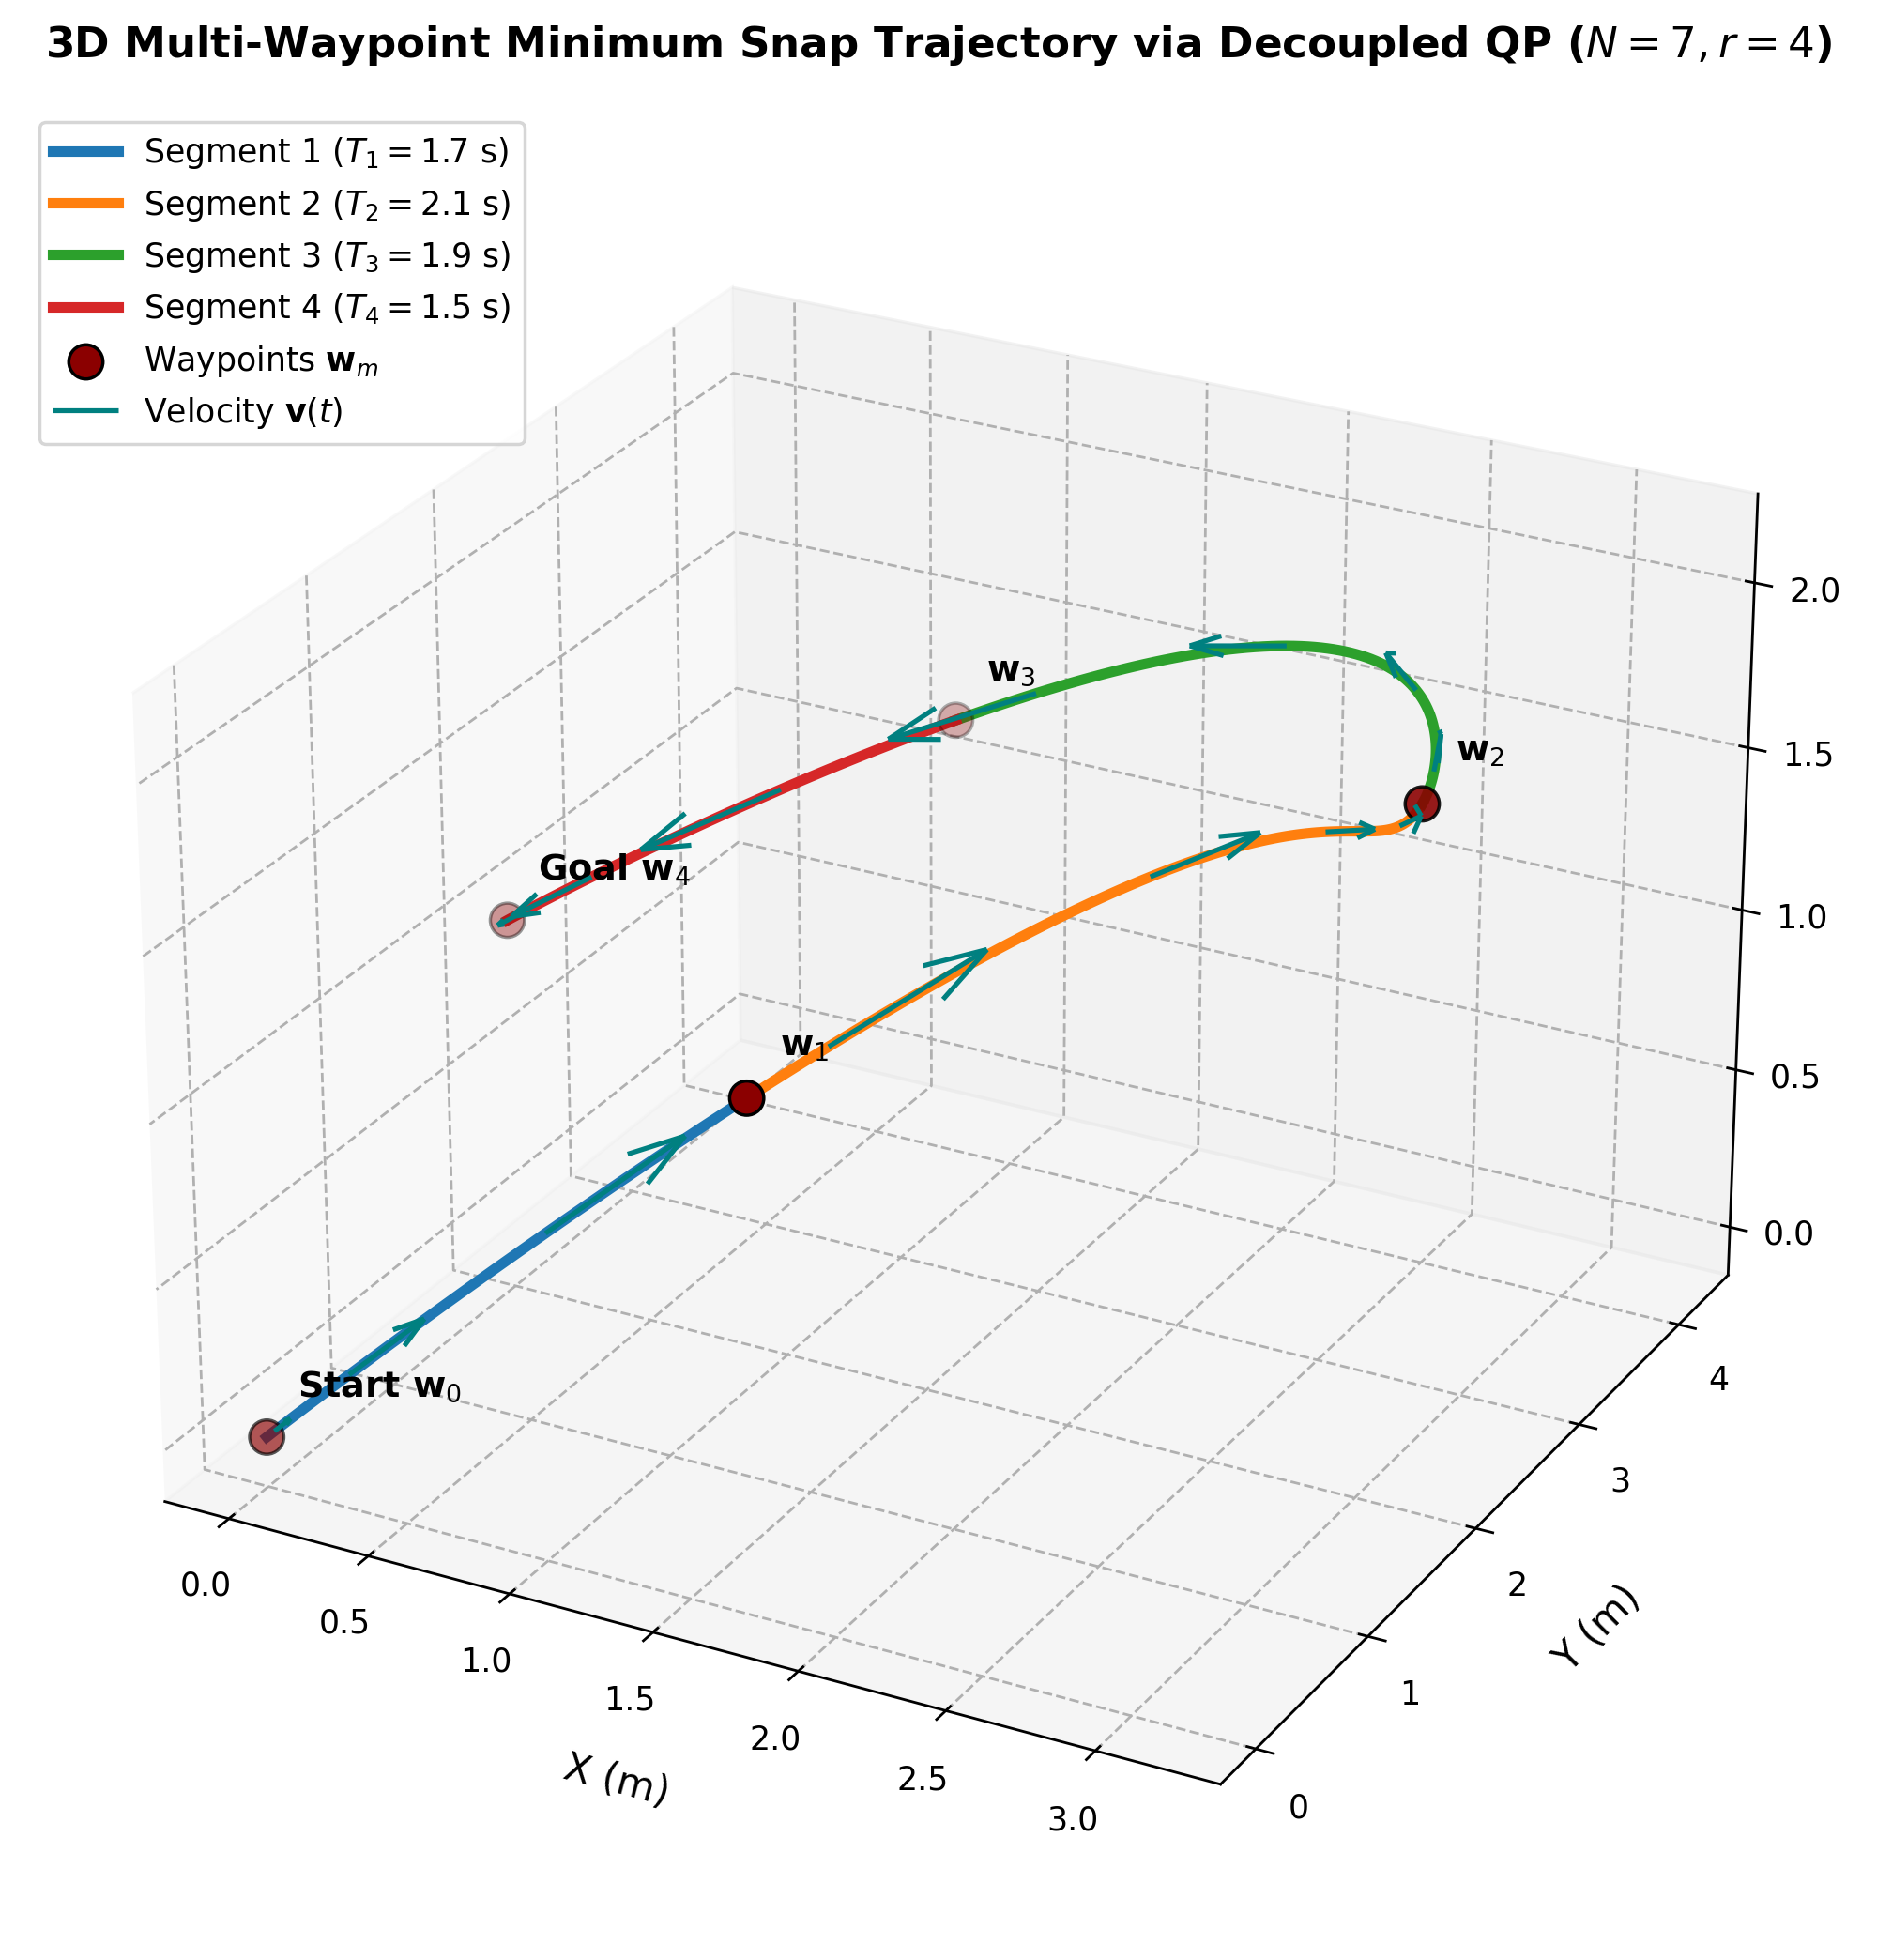
\includegraphics[width=0.92\textwidth]{multi_waypoint_3d_trajectory.png}
    \caption{\textbf{3D Multi-Waypoint Minimum Snap Flight Path}: An autonomous quadrotor trajectory visiting 5 waypoints ($\mathbf{w}_0 \to \mathbf{w}_1 \to \mathbf{w}_2 \to \mathbf{w}_3 \to \mathbf{w}_4$) across 4 polynomial segments ($N=7, r=4$). Segment durations $T_m$ are allocated proportionally to Euclidean segment lengths. Sampled velocity vectors (teal arrows) illustrate smooth directional changes through waypoints without sharp corners.}
    \label{fig:multi_waypoint_3d}
\end{figure}

\begin{figure}[H]
    \centering
    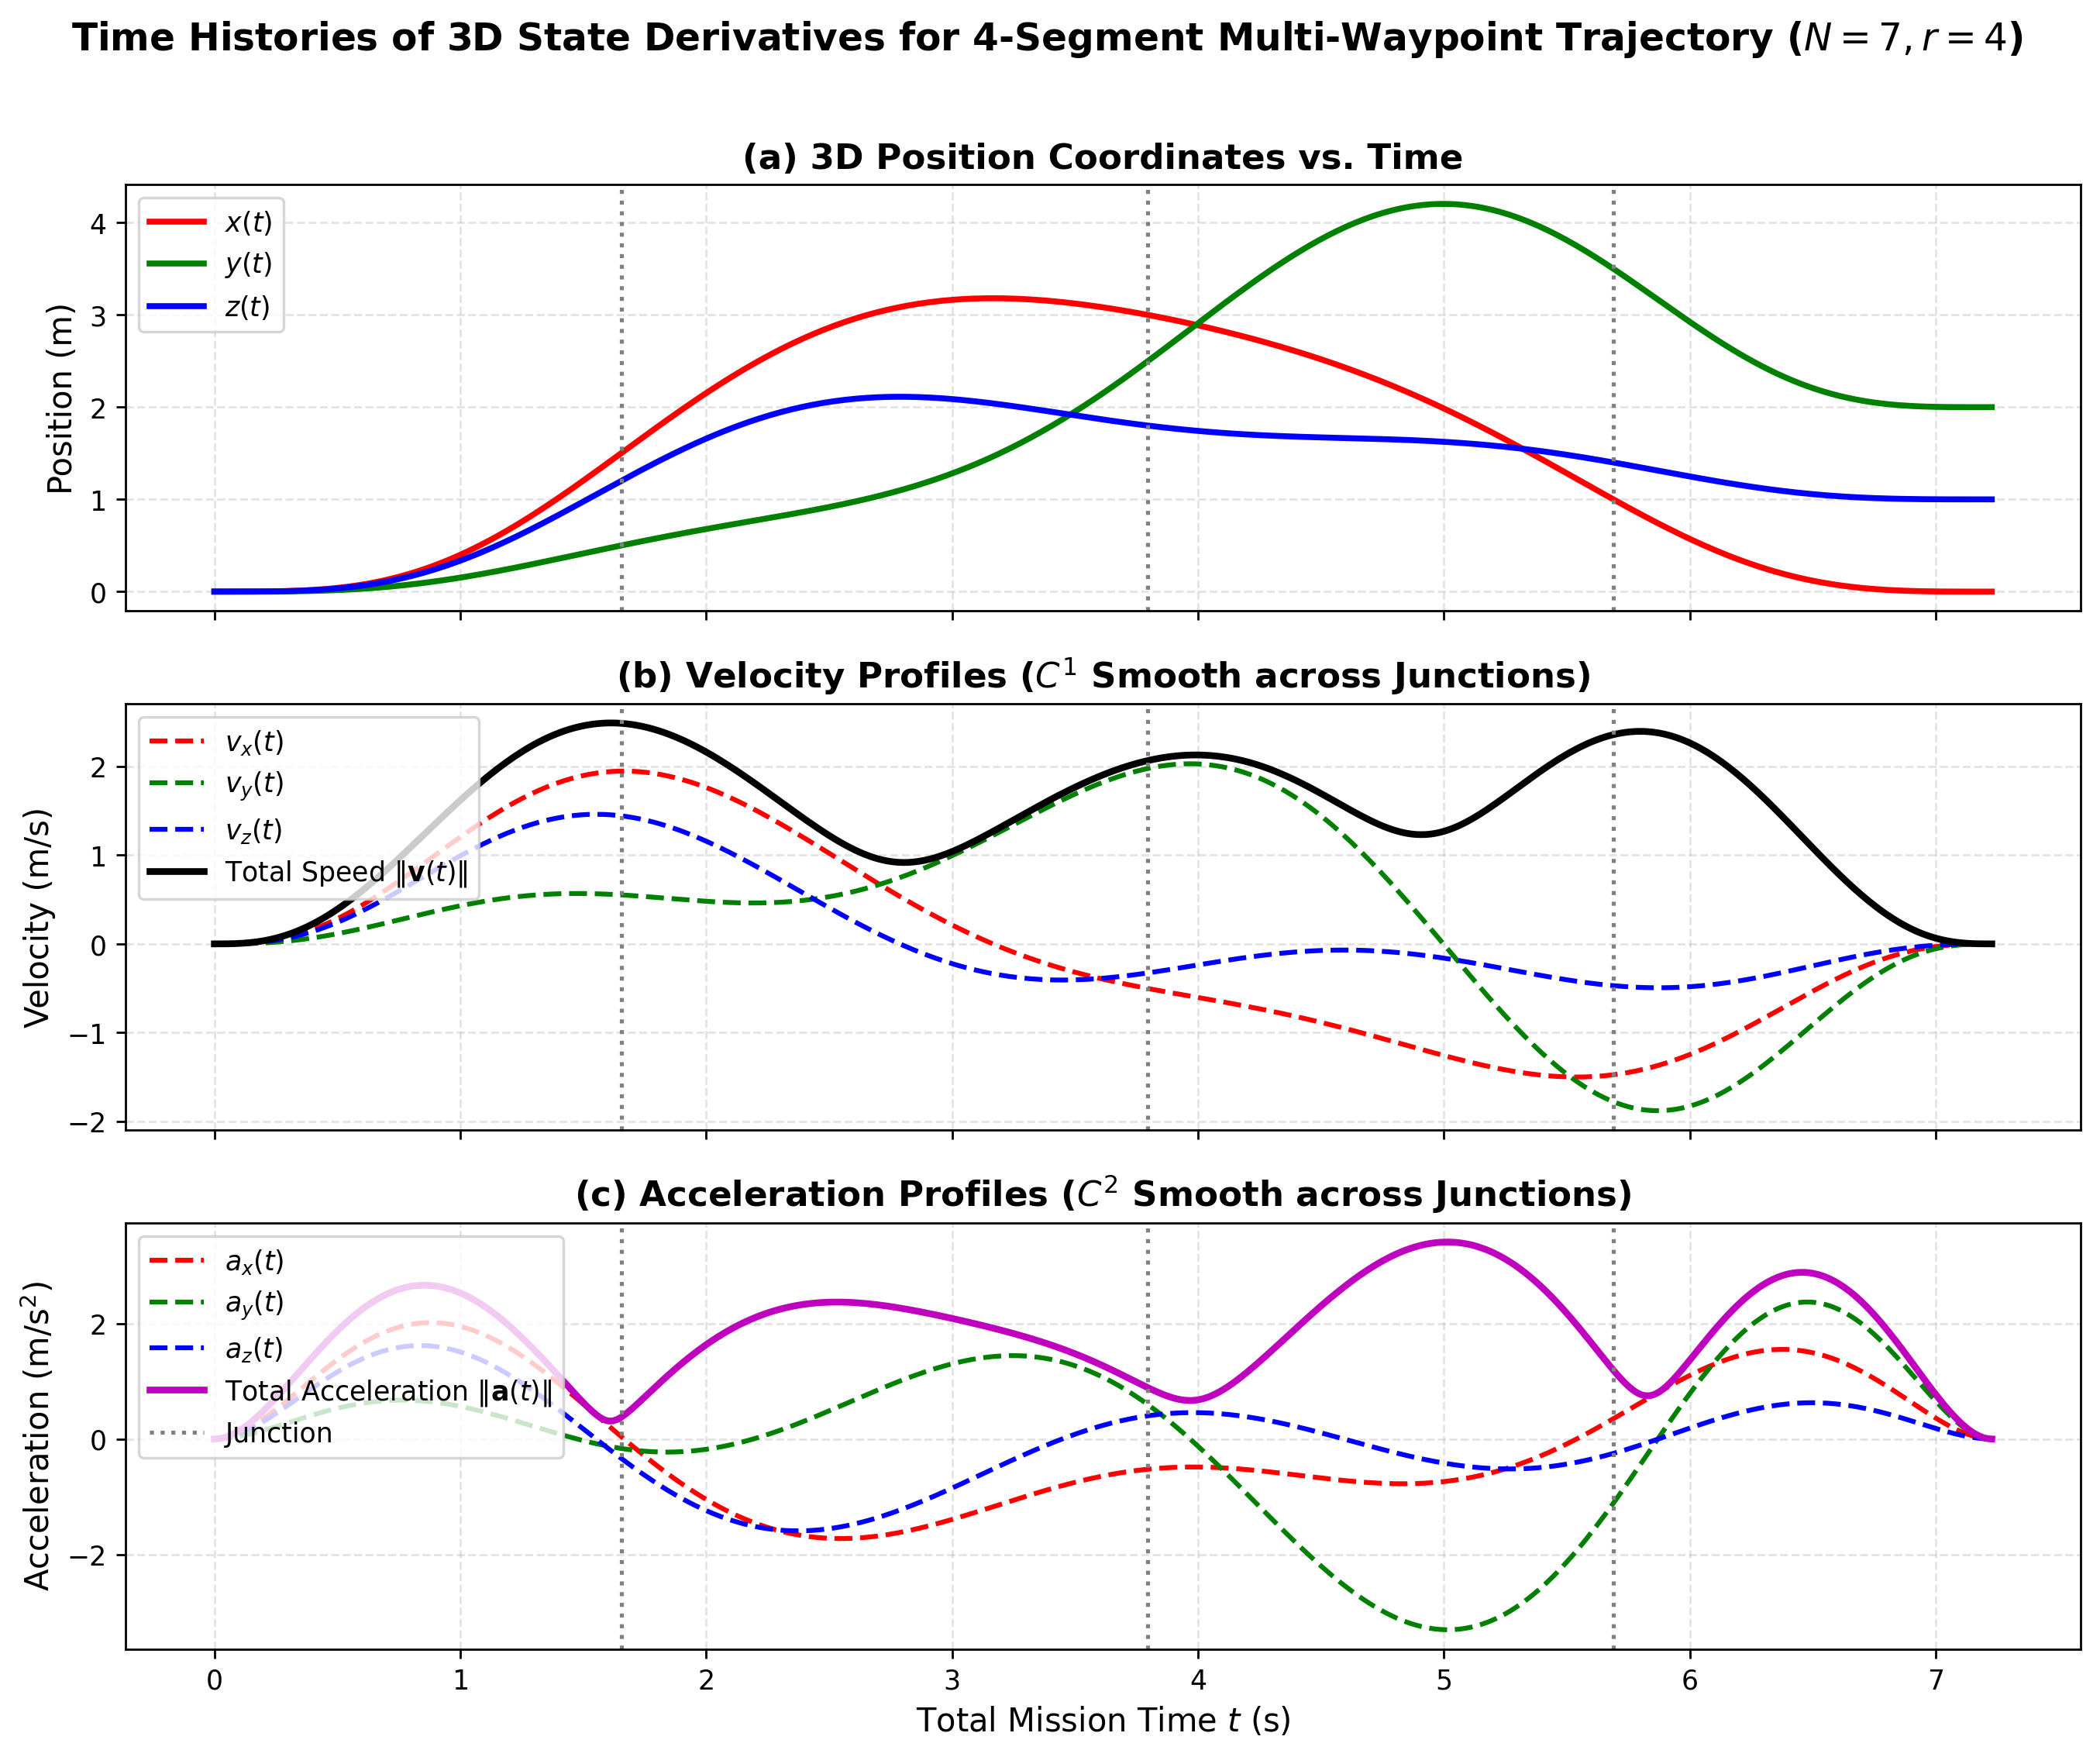
\includegraphics[width=0.95\textwidth]{multi_segment_profiles.png}
    \caption{\textbf{Time Histories of 3D Multi-Segment Flight}: 
    \textbf{(a)} Position coordinates $x(t), y(t), z(t)$.
    \textbf{(b)} Velocity components and total speed $\|\mathbf{v}(t)\|$ ($C^1$ continuous).
    \textbf{(c)} Acceleration components and total acceleration $\|\mathbf{a}(t)\|$ ($C^2$ continuous). Dotted vertical lines mark the internal segment junctions, confirming zero discontinuities across boundaries.}
    \textbf{(c)} Acceleration components and total acceleration $\|\mathbf{a}(t)\|$ ($C^2$ continuous). Dotted vertical lines mark internal segment junctions, confirming zero discontinuities across boundaries.}
    \label{fig:multi_segment_profiles}
\end{figure}

% =============================================================================
\section{Step-by-Step CVXOPT Implementation}
% =============================================================================

We now present the complete, self-contained Python implementation of the polynomial trajectory QP solver using \texttt{cvxopt}.
We now present the complete Python implementation of the equality-constrained polynomial trajectory solver using \texttt{cvxopt}.

\subsection{Matrix Construction Functions}

\begin{lstlisting}[language=Python, caption={Python/CVXOPT Implementation of Polynomial Trajectory QP Functions.}]
\begin{lstlisting}[language=Python, caption={Python/CVXOPT Implementation of Polynomial Trajectory Matrix Construction.}]
import numpy as np
import cvxopt
from cvxopt import matrix, solvers

# Mute solver progress printouts
solvers.options['show_progress'] = False

def poly_derivative_coeff(i, r):
    """Computes d^r/dt^r (t^i) scalar factor: i! / (i - r)!"""
    if i < r:
        return 0.0
    val = 1.0
    for k in range(r):
        val *= (i - k)
    return val

def compute_Q_matrix(N, r, T):
    """
    Computes (N+1) x (N+1) Hessian Q(T) for r-th derivative integral.
    Formula: Q_ij = [i!/(i-r)!] * [j!/(j-r)!] * [T^(i+j-2r+1) / (i+j-2r+1)]
    """
    Q = np.zeros((N + 1, N + 1), dtype=np.float64)
    for i in range(r, N + 1):
        for j in range(r, N + 1):
            ci = poly_derivative_coeff(i, r)
            cj = poly_derivative_coeff(j, r)
            exp_val = i + j - 2 * r + 1
            Q[i, j] = (ci * cj / exp_val) * (T ** exp_val)
    return Q

def eval_poly_basis(N, d, t):
    """Returns vector [d^d/dt^d (t^0), ..., d^d/dt^d (t^N)]^T at time t."""
    vec = np.zeros(N + 1, dtype=np.float64)
    for i in range(d, N + 1):
        ci = poly_derivative_coeff(i, d)
        vec[i] = ci * (t ** (i - d))
    return vec
\end{lstlisting}

\subsection{Multi-Waypoint Piecewise QP Solver}
\subsection{Multi-Waypoint Piecewise EQP Solver}

\begin{lstlisting}[language=Python, caption={Multi-Waypoint QP Solver in CVXOPT with Continuity Constraints.}]
\begin{lstlisting}[language=Python, caption={Multi-Waypoint Equality-Constrained QP Solver in CVXOPT.}]
def solve_multi_waypoint_qp(waypoints, segment_times, N=7, r=4):
    """
    Solves multi-segment minimum snap (r=4) trajectory for 1D waypoints.
    waypoints: list of [w_0, w_1, ..., w_M]
    segment_times: list of durations [T_1, T_2, ..., T_M]
    """
    M = len(segment_times)
    n_vars_seg = N + 1
    total_vars = M * n_vars_seg

    # 1. Construct Block-Diagonal Hessian P = 2 * blkdiag(Q_1, ..., Q_M)
    Q_tot = np.zeros((total_vars, total_vars), dtype=np.float64)
    for m in range(M):
        Qm = compute_Q_matrix(N, r, segment_times[m])
        idx = m * n_vars_seg
        Q_tot[idx:idx + n_vars_seg, idx:idx + n_vars_seg] = Qm

    P_mat = matrix(2.0 * Q_tot)
    q_mat = matrix(np.zeros(total_vars, dtype=np.float64))

    # 2. Construct Equality Constraints: A_eq * c = b_eq
    # 2. Construct Equality Constraints: A * c = b
    A_rows, b_rows = [], []

    # (a) Waypoint passage constraints for each segment
    for m in range(M):
        idx = m * n_vars_seg
        Tm = segment_times[m]

        # p_m(0) = w_m
        row_start = np.zeros(total_vars)
        row_start[idx:idx + n_vars_seg] = eval_poly_basis(N, 0, 0.0)
        A_rows.append(row_start)
        b_rows.append(waypoints[m])

        # p_m(T_m) = w_{m+1}
        row_end = np.zeros(total_vars)
        row_end[idx:idx + n_vars_seg] = eval_poly_basis(N, 0, Tm)
        A_rows.append(row_end)
        b_rows.append(waypoints[m + 1])

    # (b) Mission boundary conditions at start and end: v=a=j=0
    for d in range(1, r):
        # Start at rest
        row_init = np.zeros(total_vars)
        row_init[0:n_vars_seg] = eval_poly_basis(N, d, 0.0)
        A_rows.append(row_init)
        b_rows.append(0.0)

        # End at rest
        row_final = np.zeros(total_vars)
        row_final[(M - 1) * n_vars_seg:] = eval_poly_basis(N, d, segment_times[-1])
        A_rows.append(row_final)
        b_rows.append(0.0)

    # (c) Inter-segment continuity constraints: p_m^(d)(T_m) = p_{m+1}^(d)(0)
    for m in range(M - 1):
        idx_m = m * n_vars_seg
        idx_next = (m + 1) * n_vars_seg
        Tm = segment_times[m]
        for d in range(1, r + 1):
            row_cont = np.zeros(total_vars)
            row_cont[idx_m:idx_m + n_vars_seg] = eval_poly_basis(N, d, Tm)
            row_cont[idx_next:idx_next + n_vars_seg] = -eval_poly_basis(N, d, 0.0)
            A_rows.append(row_cont)
            b_rows.append(0.0)

    A_mat = matrix(np.array(A_rows, dtype=np.float64))
    b_mat = matrix(np.array(b_rows, dtype=np.float64))

    # 3. Solve Convex QP via CVXOPT primal-dual interior-point method
    # 3. Solve Pure Equality-Constrained QP via CVXOPT
    # Pass None for G and h matrices:
    sol = solvers.qp(P_mat, q_mat, None, None, A_mat, b_mat)
    c_tot = np.array(sol['x']).flatten()

    # Partition back into segment-wise coefficients
    c_segs = [c_tot[m * n_vars_seg:(m + 1) * n_vars_seg] for m in range(M)]
    return c_segs
\end{lstlisting}

% =============================================================================
\section{Summary and Key Takeaways}
% =============================================================================

\begin{table}[H]
\centering
\caption{\textbf{Comprehensive Summary of Polynomial Trajectory Optimization}.}
\caption{\textbf{Comprehensive Summary of Equality-Constrained Polynomial Trajectory Optimization}.}
\vspace{0.5em}
\resizebox{\textwidth}{!}{%
\begin{tabular}{@{}llll@{}}
\toprule
\textbf{Feature} & \textbf{Minimum Acceleration ($r=2$)} & \textbf{Minimum Jerk ($r=3$)} & \textbf{Minimum Snap ($r=4$)} \\
\midrule
\textbf{Minimizes} & Inertial forces \& kinetic energy & Rate of change of tilt & Rotor torques \& bandwidth \\
\textbf{Natural Degree} & Cubic ($N=3$) & Quintic ($N=5$) & Septic ($N=7$) \\
\textbf{Cost Scaling Law} & $J^*(T) \propto T^{-3}$ & $J^*(T) \propto T^{-5}$ & $J^*(T) \propto T^{-7}$ \\
\textbf{Peak Velocity} & $v_{\max} \propto T^{-1}$ & $v_{\max} \propto T^{-1}$ & $v_{\max} \propto T^{-1}$ \\
\textbf{Peak Acceleration} & $a_{\max} \propto T^{-2}$ & $a_{\max} \propto T^{-2}$ & $a_{\max} \propto T^{-2}$ \\
\textbf{Boundary Jerk} & Discontinuous at boundaries & Discontinuous at boundaries & Smooth ($j(0)=j(T)=0$) \\
\textbf{CVXOPT Solution} & Interior-point ($<0.5\,\text{ms}$) & Interior-point ($<0.5\,\text{ms}$) & Interior-point ($<1.0\,\text{ms}$) \\
\textbf{Minimizes} & Inertial forces \& kinetic energy & Rate of change of body tilt & Rotor torque bandwidth \\
\textbf{Natural Minimal Degree} & Cubic ($N=3$) & Quintic ($N=5$) & Septic ($N=7$) \\
\textbf{Cost Scaling Law} & $J^*(T) \propto T^{-3}$ & $J^*(T) = \frac{720 \Delta p^2}{T^5} \propto T^{-5}$ & $J^*(T) \propto T^{-7}$ \\
\textbf{Peak Velocity Scaling} & $v_{\max} \propto T^{-1}$ & $v_{\max} \propto T^{-1}$ & $v_{\max} \propto T^{-1}$ \\
\textbf{Peak Acceleration Scaling} & $a_{\max} \propto T^{-2}$ & $a_{\max} \propto T^{-2}$ & $a_{\max} \propto T^{-2}$ \\
\textbf{Boundary Jerk} & Discontinuous at boundaries & Non-zero at boundaries & Smooth ($j(0)=j(T)=0$) \\
\textbf{Closed-Form Solution} & Direct KKT Inverse & Direct KKT Inverse & Direct KKT Inverse \\
\textbf{CVXOPT EQP Solve Time} & $<0.2\,\text{ms}$ & $<0.2\,\text{ms}$ & $<0.3\,\text{ms}$ \\
\bottomrule
\end{tabular}%
}
\end{table}

\begin{examplebox}[Summary of Key Insights]
\begin{enumerate}
    \item \textbf{Flatness is the Key Enabler}: Quadrotor dynamics allow converting complex non-linear 6-DOF trajectory optimization into simple uncoupled polynomial curve generation in $x(t), y(t), z(t)$.
    \item \textbf{Flatness Converts Dynamics into Curves}: Quadrotor dynamics allow converting complex non-linear 6-DOF trajectory optimization into three uncoupled polynomial curve generations in $x(t), y(t), z(t)$.
    \item \textbf{Analytical Hessian Computation}: The cost matrix $\mathbf{Q}(T)$ can be computed in closed form using Eq.~\eqref{eq:Q_formula} without numerical quadrature errors.
    \item \textbf{Power-Law Time Scaling}: Duration $T$ has a dramatic non-linear effect on trajectory cost ($T^{-(2r-1)}$) and peak accelerations ($T^{-2}$). Setting $T$ too small causes immediate motor saturation; setting $T$ based on physical limits $T \ge \max(c_v \Delta p / v_{\lim}, \sqrt{c_a \Delta p / a_{\lim}})$ guarantees actuator feasibility.
    \item \textbf{Seamless Piecewise Extension}: Multi-waypoint missions are formulated by stacking segment blocks into a block-diagonal QP. Enforcing $C^3$ and $C^4$ continuity yields glass-smooth flights through complex 3D environments.
    \item \textbf{Closed-Form KKT Inversion}: Focusing on equality constraints yields a linear KKT system $\begin{bmatrix} 2\mathbf{Q} & \mathbf{A}^T \\ \mathbf{A} & \mathbf{0} \end{bmatrix} \begin{bmatrix} \mathbf{c}^* \\ \boldsymbol{\nu}^* \end{bmatrix} = \begin{bmatrix} \mathbf{0} \\ \mathbf{b} \end{bmatrix}$, which has a direct closed-form solution solvable in microseconds.
    \item \textbf{Exact Quintic Derivation}: For minimum jerk with 6 boundary conditions, degree $N=5$ yields the exact canonical trajectory $p(t) = \frac{15}{4}t^3 - \frac{45}{16}t^4 + \frac{9}{16}t^5$ for a unit transition. Over-parameterizing with $N=6$ automatically zeroes out the 6th degree coefficient $c_6 = 0$.
    \item \textbf{Power-Law Time Scaling}: Duration $T$ has a dramatic non-linear effect on trajectory cost ($T^{-(2r-1)}$) and peak accelerations ($T^{-2}$). Setting $T$ based on physical limits $T \ge \max(c_v \Delta p / v_{\lim}, \sqrt{c_a \Delta p / a_{\lim}})$ guarantees actuator feasibility without requiring numerical inequality iterations.
    \item \textbf{Seamless Piecewise Extension}: Multi-waypoint missions are formulated by stacking segment blocks into a block-diagonal EQP. Enforcing $C^3$ and $C^4$ continuity yields glass-smooth flights through complex 3D environments.
\end{enumerate}
\end{examplebox}

\begin{thebibliography}{9}
\bibitem{mellinger2011}
D.~Mellinger and V.~Kumar, ``Minimum snap trajectory generation and control for quadrotors,'' in \emph{IEEE International Conference on Robotics and Automation (ICRA)}, pp.~2520--2525, 2011.

\bibitem{fliess1995}
M.~Fliess, J.~L{\'e}vine, P.~Martin, and P.~Rouchon, ``Flatness and defect of non-linear systems: introductory theory and examples,'' \emph{International Journal of Control}, vol.~61, no.~6, pp.~1327--1361, 1995.

\bibitem{richter2016}
C.~Richter, A.~Bry, and N.~Roy, ``Polynomial trajectory planning for aggressive flight with obstacle avoidance,'' in \emph{Robotics Research}, Springer, pp.~435--451, 2016.

\bibitem{boyd2004}
S.~Boyd and L.~Vandenberghe, \emph{Convex Optimization}, Cambridge University Press, 2004.
\end{thebibliography}

\end{document}
